%%
%% This is file `elsarticle-template-num.tex',
%% generated with the docstrip utility.
%%
%% The original source files were:
%%
%% elsarticle.dtx  (with options: `numtemplate')
%% 
%% Copyright 2007, 2008 Elsevier Ltd.
%% 
%% This file is part of the 'Elsarticle Bundle'.
%% -------------------------------------------
%% 
%% It may be distributed under the conditions of the LaTeX Project Public
%% License, either version 1.2 of this license or (at your option) any
%% later version.  The latest version of this license is in
%%    http://www.latex-project.org/lppl.txt
%% and version 1.2 or later is part of all distributions of LaTeX
%% version 1999/12/01 or later.
%% 
%% The list of all files belonging to the 'Elsarticle Bundle' is
%% given in the file `manifest.txt'.
%% 

%% Template article for Elsevier's document class `elsarticle'
%% with numbered style bibliographic references
%% SP 2008/03/01

\documentclass[authoryear,preprint,12pt]{elsarticle}

%% Use the option review to obtain double line spacing
%% \documentclass[authoryear,preprint,review,12pt]{elsarticle}

%% Use the options 1p,twocolumn; 3p; 3p,twocolumn; 5p; or 5p,twocolumn
%% for a journal layout:
%% \documentclass[final,1p,times]{elsarticle}
%% \documentclass[final,1p,times,twocolumn]{elsarticle}
%% \documentclass[final,3p,times]{elsarticle}
%% \documentclass[final,3p,times,twocolumn]{elsarticle}
%% \documentclass[final,5p,times]{elsarticle}
%% \documentclass[final,5p,times,twocolumn]{elsarticle}

%% if you use PostScript figures in your article
%% use the graphics package for simple commands
%% \usepackage{graphics}
%% or use the graphicx package for more complicated commands
\usepackage{graphicx}
%% or use the epsfig package if you prefer to use the old commands
%% \usepackage{epsfig}

%% The amssymb package provides various useful mathematical symbols
\usepackage{amsmath,amssymb,color}
%% The amsthm package provides extended theorem environments
%% \usepackage{amsthm}
%% \usepackage{showlabels}
%% The lineno packages adds line numbers. Start line numbering with
%% \begin{linenumbers}, end it with \end{linenumbers}. Or switch it on
%% for the whole article with \linenumbers.
%% \usepackage{lineno}

\newcommand{\commentSofia}[1]{\vspace{1 mm}\par
  \marginpar{\large\underline{}}\noindent
  \framebox{\begin{minipage}[c]{0.95 \textwidth}
      \color{blue}\bfseries SOFIA SAYS: #1 \end{minipage}}\vspace{2 mm}\par}
\newcommand{\commentBrandon}[1]{\vspace{1 mm}\par
  \marginpar{\large\underline{}}\noindent
  \framebox{\begin{minipage}[c]{0.95 \textwidth}
      \color{red}\bfseries BRANDON SAYS: #1 \end{minipage}}\vspace{2 mm}\par}
\newcommand{\commentGareth}[1]{\vspace{1 mm}\par
  \marginpar{\large\underline{}}\noindent
  \framebox{\begin{minipage}[c]{0.95 \textwidth}
      \color{green}\bfseries GARETH SAYS: #1 \end{minipage}}\vspace{2 mm}\par}

\DeclareMathOperator*{\argmax}{arg\,max}
\DeclareMathOperator*{\argmin}{arg\,min}
\newcommand{\var}{\text{Var}}
\newcommand{\cov}{\text{Cov}}
\newcommand{\HOT}{\text{HOT}}
\newcommand{\E}{\text{E}}
\newcommand{\re}{\text{re}}
\newcommand{\im}{\text{im}}
\newcommand{\be}{\mathbf{e}}
\newcommand{\bp}{\mathbf{p}}
\newcommand{\bq}{\mathbf{q}}
\newcommand{\bd}{\mathbf{d}}
\newcommand{\bD}{\mathbf{D}}
\newcommand{\bE}{\mathbf{E}}
\newcommand{\bF}{\mathbf{F}}
\newcommand{\q}{\mathbf{q}}
\newcommand{\Q}{\mathbf{Q}}
\newcommand{\br}{\mathbf{r}}
\newcommand{\bsL}{\bs{\Lambda}}
\newcommand{\bsS}{\bs{\Sigma}}
\newcommand{\bsu}{\bs{\upsilon}}
\newcommand{\x}{\mathbf{x}}
\newcommand{\X}{\mathbf{X}}
\newcommand{\y}{\mathbf{y}}
\newcommand{\bbC}{\mathbb{C}}
\newcommand{\cA}{\mathcal{A}}
\newcommand{\cF}{\mathcal{F}}
\newcommand{\cG}{\mathcal{G}}
\newcommand{\cH}{\mathcal{H}}
\newcommand{\cI}{\mathcal{I}}
\newcommand{\cK}{\mathcal{K}}
\newcommand{\cQ}{\mathcal{Q}}
\newcommand{\cP}{\mathcal{P}}
\newcommand{\bbR}{\mathbb{R}}
\newcommand{\cR}{\mathcal{R}}
\newcommand{\cS}{\mathcal{S}}
\newcommand{\cZ}{\mathcal{Z}}
\newcommand{\eps}{\epsilon}
\newcommand{\vare}{\varepsilon}
\newcommand{\bld}[1]{\mathbf{#1}}
\newcommand{\bs}[1]{\boldsymbol{#1}}
\newcommand{\wh}[1]{\widehat{#1}}
\newcommand{\wt}[1]{\widetilde{#1}}
\newcommand{\ol}[1]{\overline{#1}}

\journal{NeuroImage}
%\usepackage{datetime}
\begin{document}

\begin{frontmatter}

%% Title, authors and addresses

%% use the tnoteref command within \title for footnotes;
%% use the tnotetext command for theassociated footnote;
%% use the fnref command within \author or \address for footnotes;
%% use the fntext command for theassociated footnote;
%% use the corref command within \author for corresponding author footnotes;
%% use the cortext command for theassociated footnote;
%% use the ead command for the email address,
%% and the form \ead[url] for the home page:
%% \title{Title\tnoteref{label1}}
%% \tnotetext[label1]{}
%% \author{Name\corref{cor1}\fnref{label2}}
%% \ead{email address}
%% \ead[url]{home page}
%% \fntext[label2]{}
%% \cortext[cor1]{}
%% \address{Address\fnref{label3}}
%% \fntext[label3]{}

\title{Parametric Models for Complex-Valued HARDI Data}

%% use optional labels to link authors explicitly to addresses:
%% \author[label1,label2]{}
%% \address[label1]{}
%% \address[label2]{}

\author[label1]{Sofia C. Olhede\corref{cor1}}
\ead{s.olhede@ucl.ac.uk}

\author[label2]{Gareth J. Barker}

\author[label3]{Rexford D. Newbould}

\author[label3]{Brandon Whitcher}

\cortext[cor1]{Corresponding author.}
\address[label1]{Department of Statistical Science, University
  College, London, United Kingdom}
\address[label2]{King's College London, Institute of Psychiatry,
  Department of Clinical Neuroscience, Centre for Neuroimaging
  Sciences, London, United Kingdom}
\address[label3]{Clinical Imaging Centre, GlaxoSmithKline, London,
  United Kingdom}

\begin{abstract}
Diffusion-weighted magnetic resonance imaging (DW-MRI) data are the
noisy observations of the Fourier transform (FT) from a diffusion
probability density function (PDF).  If the diffusion PDF is symmetric
in space then the DW-MRI measurements are (theoretically) real-valued;
while if the PDF exhibits some asymmetry in space then the DW-MRI
measurements are (theoretically) Hermitian complex-valued.  A model
for the complex-valued FT of the diffusion~PDF is introduced in this
paper from the three-dimensional Bolzmann equation, suitable for
complex-valued high angular resolution diffusion imaging measurements.
This model, corresponding to the characteristic function of the PDF,
may be expanded in terms of cumulants of the PDF that are functions of
its moments.  The equation therefore characterizes the PDF in terms of
its moments, where the latter can be directly related to physical
characteristics of the diffusion~PDF.  The structure of the PDF of an
idealized bending or forking fibre we argue that bending fibers
produce ``near-linear'' phase functions over a range of $q$-values,
the sphere of diffusion encoding directions, without corresponding to
net transport.  {\bf Gareth = This sentence got lost somewhere in the
  middle!}  To estimate such complex-valued structure from HARDI
observations, spurious phase is first removed from the data via a
pre-processing step.
% and information from multiple receiver coils or channels is combined
% to yield stable estimates of local phase.  A hypothesis test is
% developed to determine if the pre-processing was successful, or if
% the mean phase of measurements at a given voxel is still non-zero.
Voxels that are not Hermitian symmetric are removed from subsequent
analysis.  For such voxels, for which the pre-processing was
successful, a locally linear phase is estimated using least squares,
an estimate from which we argue the axes of locally linear asymmetry
in the diffusion~PDF may be determined if the Hermitian structure
differs significantly from the noise.  We propose analytic asymmetric
models for PDFs, discuss bending and forking in detail, and show the
performance of our method on simulated and \textit{in vivo} data
acquired from a typical clinical setting.
% We also analyse in vivo data, showing the existence of asymmetric
% structure under such conditions, and discuss the potential
% interpretation of the discovered structures.
\end{abstract}

\begin{keyword}
%% keywords here, in the form: keyword \sep keyword

%% PACS codes here, in the form: \PACS code \sep code

%% MSC codes here, in the form: \MSC code \sep code
%% or \MSC[2008] code \sep code (2000 is the default)
DTI \sep phase \sep diffusion \sep brain \sep non-Gaussian.
\end{keyword}

\end{frontmatter}

%% \linenumbers

%% main text
%\today\quad   \currenttime

\section{Introduction}
\label{intro}

High angular resolution diffusion imaging (HARDI) data has had a great
impact on the understanding of complex white-matter microstructure.
From HARDI data it is possible to estimate properties of the local
spatial diffusion of water molecules via the diffusion probability
density function (PDF).  HARDI data corresponds to multiple images
acquired with different diffusion encoding directions at a high
$b$-value, as well as at a low or zero $b$ value, and this collection
of images may be used to deduce orientational structure in the spatial
domain.  The $b$-value quantifies the influence of the
diffusion-encoding gradients on the acquired images, and is a function
of the strength of the gradient pulses, their duration as well as the
time between pulses.  HARDI data are often collected at a higher
$b$-value than is normal for diffusion tensor imaging (DTI), to
enhance any directional structure although collecting data at higher
values of $b$ reduces the SNR (signal-to-noise ratio) of the
observations.  HARDI observations are Fourier domain information and
must be converted into spatial information, usually by an
approximation to an inverse Fourier transform (IFT).  To be able to
make the necessary inversion, additional constraints must be placed on
the observed white-matter structure, as the number of observations at
each voxel fall short of the number needed for a numerically stable
IFT procedure.

A number of methods exist for the analysis of orientational structure,
with the most straightforward model corresponding to diffusion tensor
imaging (DTI) \citep{Basser1994b,Basser1994}, where a Gaussian PDF is
fitted at each voxel.  There is an analytic expression for the IFT of
the characteristic function (Fourier transform of a PDF) of a Gaussian
PDF, so the estimated parameters in $q$-space have a direct spatial
interpretation.  There are limitations to the DTI model, and to be
applicable across more heterogeneous structures either a mixture of
Gaussian PDFs must be fitted \citep{Alexander2005} or non-parametric
methods must be used.  Popular non-parametric methods include the
approach of \citet{Jansons}, corresponding to a non-parametric
estimation method of the orientational structure associated with a
single fixed spatial scale.  \citet{Tuch} proposed fully
non-parametric method of estimating spatial orientational structure
using the Funk-Radon Transform (FRT).  Improvements to the
implementation of the FRT have been proposed by \citet{Hess} and
\citet{Descoteaux}.  These are all methods of estimating an
orientational distribution function (ODF).  By an ODF we refer to any
voxel-specific representation of spatial orientational structure,
whether corresponding to a weighted average of structure across
spatial radii, or associated with a fixed radius.

It is also possible to describe more complicated heterogeneous
structure of the diffusion~PDF non-parametrically using generalized
diffusion tensors by expanding the logarithm of the characteristic
function in terms of an infinite number of higher-order terms
\citep{Ozarslan03,Liu2005,Liu2004}.  Care must be taken to
appropriately normalize the higher order moments by $b$
\cite{Liu2005}.  Practical application of such ideas corresponds to
diffusion kurtosis imaging (DKI), where the non-Gaussian higher-order
structure of the PDF is quantified \citep{Jensen2005,Lu2006,Hui2008}.
In DKI a tensor is calculated using higher-order terms in the
Kramer-Moyal expansion of the three-dimensional Bolzmann equation, and
yields additional information about the directional structure of the
diffusion~PDF.  In \citet{Lazar} an ODF was calculated directly from
the estimated diffusion tensor and diffusion kurtosis values.
% Higher-order terms may improve the representation of non-Gaussian
% features of the diffusion process \citep{Lazar}.
The higher-order terms are necessary to resolve low crossing angles
and provide information about the high-frequency components of the ODF
\citep{laz:mapping}.

All of the methods previously discussed
% ignore the fact that MRI observations are {\em complex-valued} when
% acquired off the scanner.
focus on magnitude MRI data, and ignore the phase information from the
inherently complex-valued MR acquisitions.  It has been proposed that
movement, susceptibility effects, and other random offsets to the
phase, diminish any advantage in analysing the complex-valued
observations directly.  Notable exceptions include \citet{Liu2005},
\citet{Aksoyetal2008} and \citet{Newbould}.  Arguments have been made
for the case that DW-MRI measurements are inherently real-valued and
positive \citep{Wedeen05}, thus eliminating the need to study the
complex-valued MRI data other than, for example, the goal of noise
suppression.

It is our aim to design statistical methodology for complex-valued
HARDI ($\bbC$-HARDI) data that recognize voxels where the diffusion
process does not appear to be symmetric.  Such information may be used
directly as an imaging biomarker for disease progression or treatment
response, or as an input to fiber-tracking algorithms
\citep{laz:mapping,chu-cho-che:principles}.  We also note that
analyzing complex-valued MRI measurements has recently been proposed
in the functional MRI (fMRI) literature.  Several papers by Rowe and
colleagues have proposed to retrieve biological information from the
phase of fMRI data \citep{Rowe2004,Rowe2005,Rowe2007}.  The phase
structure in fMRI may be due to vascular effects \citep{Menon} or
neuronal effects \citep{Bodurka}.

Including higher-order terms from the Kramer-Moyal expansion of the
three-dimensional Bolzmann equation implies that even and odd powers
of $q$ \textbf{[Has $q$ been define?]} feature in the expansion.  It
has been shown that any asymmetry in the diffusion~PDF leads to
complex-valued observations in $q$-space, or equivalently odd terms in
the Kramer-Moyal expansion \citep{Liu2005}.  Estimation of such terms
requires ($\bbC$-HARDI) measurements.  Acquiring observations at a
single non-zero magnitude of $b$, over the entire sphere (i.e., a
single shell), one may estimate only a single linear term in the
expansion, just as estimating higher-order even-numbered moments
requires several shells.  This does not mean we believe in net
transport at a given voxel, but the higher-order asymmetric effects in
the three-dimensional Bolzmann equation may be approximated by a
linear term, over a range of $q$-values.  Determining asymmetry is
important for better characterisation of local structure.  The ability
to distinguish forking, or bending, versus crossing fibers may depend
on the use of complex-valued observations \citep{Liu2005}.

Before interpreting the observed phase in DW-MRI we must model and
understand phase contributions that will be observed at the voxel
level and on given receiver channel (i.e., a receiver coil and its
associated electronics), although the underlying causes will be
different from the fMRI case.  For simplicity, we refer to all
elements involved in receiving the signal as a ``coil.''  We assume
that multiple complex-valued measurements are made at each coil and we
aim to estimate the phase and amplitude of the diffusion~PDF from such
measurements.  Following \citet{Aksoyetal2008} we model
movement-induced phase as affecting the smooth components of the data
in a given axial slice (\textit{x-y} plane), permitting us to remove
such effects.  Remaining phase perturbations are either attributed to
an imperfect procedure for removing the movement phase or
susceptibility effects, as well as eddy-current effects, or genuine
phase structure.  Phase effects are both subject dependent
susceptibility effects, that can be determined from the $b=0$ images,
as well as eddy current induced inhomogeneities that may be detected
when using diffusion-weighted $(b\neq{0})$ measurements.  The eddy
currents are not subject dependent \citep{Truong2008}.  Once the bias
due to movement has been removed from each coil, a weighted average is
formed to estimate the diffusion PDF phase in $q$-space, and a simple
sum is subsequently used to estimate the amplitude of the diffusion
PDF.  This yields a single amplitude and a single phase for each voxel
and diffusion encoding gradient direction.

If there are no susceptibility effects to remove, then the phase must
observe constraints from the Hermitian symmetry of the data.  The
phase at $b=b'$, the nonzero $b$-value over which $q$-space shell
measurements have been collected, should have a zero ``shell
average.''  We may test whether this null hypothesis may be rejected.
If the zero average of the phase is not rejected at $b>0$, then we
assume that the raw phase has been appropriately processed to remove
artifacts.  We estimate the coefficient of a Taylor expansion of the
three-dimensional Bolzmann equation, and test for significant
Hermitian structure.  If this is the case, then we may estimate the
Hermitian structure and try to determine what additional information
this may give us regarding the asymmetry of the diffusion PDF.

We discuss theoretical PDFs which will lead to Hermitian (complex)
structure in $q$-space and introduce analytical models for bending and
forking fibers.  We show voxels identified in $\bbC$-HARDI data,
acquired using clinical settings, that possess Hermitian structure
have a similar appearance in $q$-space to theoretical models of
diffusion~PDFs, and discuss to what spatial structure this would
correspond.  Given our extensive simulation studies, as well as
analysis of clinical data, we believe there is clear evidence of the
utility in the phase information from $\bbC$-HARDI data.

\section{Theory}

\subsection{Modelling complex-valued HARDI observations}
\label{modelling}

At any location $\x_n$, gradient $\q_l$ we define the $q$-space
observation
\begin{equation}\label{qxeqn}
  Z(\q_l;\x_n) = \cZ(\q_l;\x_n) + \eps(\q_l;\x_n) \equiv
  A(\q_l;\x_n) \exp\left(-i\phi(\q_l;\x_n)\right),
\end{equation}
$n=1,\dots,N^2$, $l=1,\dots,L$, where $\cZ(\q_l,\x_n)$ is the noise
free (complex-valued) diffusion process and $\eps(\q_l;\x_n)$ is
complex proper\footnote{This comment is strictly speaking not true.
  Since we would like to reduce acquisition time, the full pass-band
  is not sampled equally.  This makes the noise structure more
  complicated, but we may ignore this slight inaccuracy.}  Gaussian
noise with variance $\sigma^2(\x_n)$, uncorrelated in both indices $l$
and $n$, and constant in magnitude over the directions $l$
\citep{Picinbono1996}.  We assume that for $l=1,\dots,L_0$, the
observations are collected at $b=0$, and for $l=L_0+1,\dots,L$, the
observations are collected at $b=b'>0$.  To facilitate exposition we
introduce the polar decomposition
\begin{equation}
  \cZ(\q_l) = \cA(\q_l) \exp\left(-i\varphi(\q_l)\right)
\end{equation}
of the noise-free observations, where $\cA(\q_l;\x_n)$ and
$\varphi(\q_l;\x_n)$ denote the amplitude and phase terms,
respectively.  We need to model the structure of this object in terms
of gradient directions $l$.  The process $\cZ(\q_l;\x_n)$ is the
Fourier transform (FT) of the spatial PDF (probability density
function) at location $\x_n$, given by
\begin{equation}
  a(\x) = \int_{\bbR^3} \cZ(\q;\x_n) \exp\left(2i\pi\x^T\q\right) \,
  d^3 \q,
\end{equation}
where we have dropped the explicit dependence upon $n$.  We may, in
general, write
\begin{equation}\label{eq:evenodd}
  a(\x) = a_e(\x) + a_o(\x),
\end{equation}
at a fixed voxel $\x_n$, where $a_e(\x)$ is an \textit{even} function
in $\x$, its FT being real-valued, and $a_o(\x)$ is an \textit{odd}
function in $\x$, its FT being purely imaginary when non-zero.  One
example of such a scenario would be a branching fiber, where the even
function corresponds to the fiber continuing through the voxel, and
the odd function corresponds to the new branch of the fiber.
Calculating the FT of Eq.~\eqref{eq:evenodd} gives
\begin{equation}\label{eq:evenoddF}
  \cZ(\q) = \cA_e(\q)-i \cA_o(\q) = \cA(\q)
  \exp\left(-i\varphi(\q)\right),
\end{equation}
where both $\cA_e(\q)$ and $\cA_o(\q)$ are real-valued quantities;
i.e., the FTs of $a_e(\x)$ and $ia_o(\x)$, respectively.  Thus, the
asymmetry information is encoded in the imaginary part of the
$q$-space measurements $\cZ(\q)$.

In order to proceed we require a model-based procedure to estimate the
phase of the diffusion.  Starting from the three-dimensional Boltzmann
equation we may expand the observed signal using cumulant expansions
and the Kramer-Moyal formula 
\begin{equation}\label{kramermoyal}
  \frac{\cZ(\q)}{\cZ({\mathbf{0}})} = \exp\left[-iP^{(\im)}(\q) +
  P^{(\re)}(\q) + \cdots \right].
\end{equation}
\citep{Callaghan,Liu2004,Liu2005}.  Since we are modelling the phase
and amplitude it is convenient to use the two functions
\begin{eqnarray}
  P^{(\re)}(\q) &=& -\frac{1}{2!}\sum_{l_1,l_2} D^{(2)}_{l_1,l_2}
  q_{l_1}q_{l_2} + \cdots\\ 
  P^{(\im)}(\q) &=& \sum_{l_1} D^{(1)}_{l_1} q_{l_1} - \frac{1}{3!}
  \sum_{l_1}\sum_{l_2}\sum_{l_3} D^{(3)}_{l_1,l_2,l_3} q_{l_1} q_{l_2}
  q_{l_3} + \cdots,
\end{eqnarray}
where $D^{(n)}_{\bullet}$ is the $n$th order cumulant of $\x$,
$\q=(q_{l_1},q_{l_2},q_{l_3})=\gamma\delta{G}$ with $G$ being the
applied diffusion gradient, $\gamma$ the gyromagnetic ratio and
$\delta$ the duration of the two gradient pulses used.  The terms
$P^{(\re)}(\q)$ and $P^{(\im)}(\q)$, in general, contain an infinite
number of terms and cannot be estimated from finite sample sizes of
$\bbC$-HARDI data.  To find simple expressions over a range of $\q$
values we approximate the functions using
\begin{eqnarray}
  \nonumber
  P^{(\re)}(\q) &=& -\frac{1}{2} \q^T\bD^{(\re)}\q + e^{(\re)}(\q),\\
  \nonumber
  P^{(\im)}(\q) &=& P^{(\im)}_q(\q) \quad \text{if} \quad \|\q\|=q,\\
  \label{taylor:phase2}
  P^{(\im)}_q(\q) &=& \Phi_0^{(q)} + \q^T\bd^{(\im)} + e^{(\im)}_q(\q),
\end{eqnarray}
where $\Phi_0^{(q)}$ is the phase-shift term and may pick up the
remaining bias in the data that the pre-processing steps have not
resolved (Section~\ref{preprocessing}).  The terms
\begin{eqnarray}
  \bd^{(\im)} &=& \begin{pmatrix}
    D^{(1)}_{1} & D^{(1)}_{2} & D^{(1)}_{3}
  \end{pmatrix}^T,\\
  \bD^{(\re)} &=& \begin{pmatrix}
    D_{1,1}^{(2)} & D_{1,2}^{(2)} & D_{1,3}^{(2)}\\
    D_{2,1}^{(2)} & D_{2,2}^{(2)} & D_{2,3}^{(2)}\\
    D_{3,1}^{(2)} & D_{3,2}^{(2)} & D_{3,3}^{(2)}
  \end{pmatrix},
\end{eqnarray}
provide convenient matrix notation for the first- and second-order
cumulants.  The function $e^{(\bullet)}(\q)$ is the difference between
the theoretical model and our simple approximation, and so
\begin{eqnarray}
  e^{(\im)}(\q) &=& P^{(\im)}_q(\q) - \Phi_0^{(q)} + \q^T\bd^{(\im)}\\
  e^{(\re)}(\q) &=& P^{(\re)}(\q)+\frac{1}{2} \q^T\bD^{(\re)}\q.  
\end{eqnarray}
Because the noise is added to $\cZ(\q)$ and the truncation errors
occur in $\log\cZ(\q)$ it is not necessarily advantageous to combine
them together.  Thus, we retain a simple quadratic function for the
even terms (i.e., use the standard diffusion tensor model for the even
terms), and use a linear approximation for the odd terms, suitable
when $\|\q\|=q$.  \commentSofia{This is inconsistent with our previous
  notation, $q$ was $q'$?}
% The term $\Phi_0^{(q)}$ is for the phase shift and may pick up
% remaining bias in the data that our pre-processing has not resolved
% (see~\ref{preprocessing}).

If we collect data at several values of $q$, the diffusion tensor
model for the magnitude may need augmentation with higher-order even
terms (as in diffusion kurtosis imaging).  The function
$P^{(\cdot)}(\q)$ only admits a valid interpretation over a limited
range of $q$-values.  For example, we do not believe in net transport,
but rather assume that higher-order terms are locally approximated by
the linear term.  With these equations we note that
\begin{eqnarray}\label{model}
  \log\cZ(\q) &=& \log \cA_0 - i \phi_0 - i \q^T\bd^{(\im)} -
  \frac{1}{2} \q^T\bd^{(\re)}\q + e(\q)\\  
  &=& \log \cA(\q)-i\varphi(\q),
\end{eqnarray}
where the latter equation is simply the logarithm of
Eq.~\eqref{eq:evenoddF}, and $A(\q)$ as well as $\phi(\q)$ are the
noisy (sampled) versions of $\cA(\q)$ and $\varphi(\q)$, so that
$\log{Z(\q)}=\log{A(\q)}-i\phi(\q)$.  This provides a model for the
observations and may be used to construct an estimation procedure.  If
the complex-valued measurements are real-valued, then there are no
asymmetries in the PDF and $\bd^{(\im)}\equiv\bld{0}$.  That is, there
is nothing of interest in the apparent complexity of the observations
and the likelihood may be marginalized in terms of the positive,
real-valued random variables $\{A(\q)\}$, or we may possibly reduce
noise by fitting the parametric model to $\{A_e(\q)\}$ rather than to
$\{A(\q)\}$.

\subsection{A bending fiber population model}

We now consider a model for the asymmetry of the diffusion~PDF at a
given voxel; specifically, a voxel that corresponds to a bending
structure.  In this case it makes sense to think of a single fiber
population, which is skewed (bending in space).  Unfortunately, to
connect this type of structure to the analysis of the magnitude we
have to model it as a mixture of two fiber populations and write for
\begin{equation}\label{mixture}
  \frac{\cZ(\q)}{\cZ(\bld{0})} = \alpha\frac{\cZ_1(\q)}{\cZ_1(\bld{0})}
  + (1-\alpha)\frac{\cZ_2(\q)}{\cZ_2(\bld{0})},
\end{equation}
where
$\alpha=\cZ_1(\bld{0})/[\cZ_1(\bld{0})+\cZ_2(\bld{0})]\in[0,1]$,
is the volume fraction of each branch (normally would be modelled as a
half).  
% \commentSofia{Is my usage of volume fraction correct here?}
Both $\cZ_1(\q)$ and $\cZ_2(\q)$ may be modelled as branches of fibers
(i.e., highly asymmetric diffusion PDFs) meeting at the center of the
voxel. Therefore, they are genuinely complex-valued quantities since
each branch is highly asymmetric and is modelled as entering but not
exiting the voxel.  We then have
\begin{eqnarray}
  \varphi(\q) &=& -\tan^{-1}
    \left(\frac{\alpha\Im\left\{\cZ_1(\q)/\cZ_1(\bld{0})\right\} +
    (1-\alpha) \Im\left\{\cZ_2(\q)/\cZ_2(\bld{0})\right\}}
    {\alpha\Re\left\{\cZ_1(\q)/\cZ_1(\bld{0})\right\} + (1-\alpha)
    \Re\left\{\cZ_2(\q)/\cZ_2(\bld{0})\right\}}\right).
\end{eqnarray}
This equation represents the phase structure of the entire voxel of
the characteristic function in terms of the volume fraction and the
characteristic function of each branch.  The phase of the normalized
mixture reflects the structure of both branches, depending on the
value of $\alpha$ and the value of $|\cZ_l(\q)|,$ $l=1,2$.  Note that
for most of $\q$-space only one of the two branches is non-zero.  The
phase from each of the branches is changing perpendicularly to the
great circle associated with the magnitude of the branch.  The mixture
of fiber populations have a phase which is varying parallel to the
amplitude.

To exemplify typical bending structure we first construct a single
branch by dividing a Gaussian~PDF into two halves, non-zero for
$x_1>0$ and zero for $x_1<0$ (without loss of generality).  This
corresponds to the tensor product of a half-Gaussian (or half-Normal)
distribution in $x_1$ and two Gaussian distributions in $x_2$ and
$x_3$, respectively.  We model a bending fiber by aggregating two
half-Gaussian functions with different axes of the asymmetry.  If we
used the same axes and eigenvalues we would just get back a single DTI
model without bending.  We plot the real-part, imaginary-part,
amplitude and phase for our example and a choice of parameters in
Fig.~\ref{bending}.  Observe that the phase in Figs.~\ref{bending}a
and~\ref{bending}e is nearly linear, the magnitude reflects the
two-tensor structure of the data (or equally a scalene diffusion may
be fitted from a single shell of observations), and the magnitude of
the imaginary component has similar structure to a DTI model but with
two large eigenvalues and one small eigenvalue.  \textbf{[More text is
    needed to describe the figure!!!]}  The magnitude of the real part
is also consistent with a two-tensor model or equally a scalene
diffusion for single shell observations.

The bending fiber (in general) has to show variation in the phase
mainly perpendicular to the great circle, with its zeros going though
the direction of the averages of the two populations.  Furthermore, if
we are in a voxel where $|\cZ_1(\q)|\gg|\cZ_2(\q)|$, then \textbf{[I
    have mucked around with this equation... please double check!]}
\begin{equation}
  \varphi(\q) = -\tan^{-1} \left(\frac{\alpha |\cZ_1(\q)|^{-1}
    \Im\{\cZ_1(\q)\} + (1-\alpha) |\cZ_2(\q)|^{-1} \Im\{\cZ_2(\q)\}}
         {\alpha |\cZ_1(\q)|^{-1} \Re\{\cZ_1(\q)\} + (1-\alpha)
           |\cZ_2(\q)|^{-1} \Re\{\cZ_2(\q)\}} \right) \approx
         \varphi_1(\q),
\end{equation}
namely the phase of $\cZ_1(\q)$.  To elaborate on this, if (as in the
previous example with the half-Gaussian) we constructed $\cZ_1(\q)$ by
taking a symmetric diffusion~PDF and setting half of the PDF to zero
in the direction $\bsu_1$, then $a_1(\x)=2a_{1e}(\x)I(\x^T\bsu_1>0)$,
where $ a_{1e}(\x)$ has FT $\cA_{1e}(\q)$.  We assume that
$\cA_{le}(\q)$ is an ellipsoid density with axes $\{\bsu_k\}$ for
$k=1,2,3$, while $\cA_{2e}(\q)$ is an ellipsoid density with axes
$\{\bs{\xi}_k\}$ for $k=1,2,3$.  Functions that are zero for a given
half-space are related to the partial Hilbert transform
\citep{Granlund} calculated in some set direction, and we denote the
Hilbert transform in direction $\bsu$ by $\cH_{\bsu}\{\cdot\}$.  We
define this transform (i.e., the partial Hilbert Transform in
direction $\bsu$) in space via
\begin{equation}
  \cF^{-1}\left\{\cH_{\bsu}\left\{\cA\right\}\right\}(\x) \equiv -i \,
  \text{sign}\left(\x^T\bsu\right)a_{1e}(\x).
\end{equation}
We can therefore write the characteristic function of an asymmetric
component of the bending fiber PDF as
\begin{eqnarray}
  \cA_1(\q) &=& \cA_{1e}(\q) - i \cH_{\bsu_1}\cA_{1e}(\q) \nonumber\\
  &=& \cA_{1e}(\bld{0})+\nabla \cA_{1e}(\bld{0})^T\q + \cdots - i
  \left(0 + \nabla\cH_{\bsu_1}\cA_{1e}(\bld{0})^T\q + \cdots\right) \nonumber\\
  &=& 1 + \cdots - i
  \left[\left(\nabla\cH_{\bsu_1}\cA_{1e}(\bld{0})\right)^T\q +
  \cdots\right],
\end{eqnarray}
and so
$\varphi_1(\q)\approx(\nabla\cH_{\bsu_1}\cA_{1e}(\bld{0}))^T\q$.  We
assumed that $a_{1e}(\x)$ was even in $\x$ and so its Fourier
transform is even and has a maximum at $\q=\bld{0}$.  This implies
that $(\nabla\cH_{\bsu_1}\cA_{1e}(\bld{0}))^T$ is proportional to
$\bsu_1$ and with $\nabla_{\bsu}$ denoting the directional derivative
in direction $\bsu$, we may write down the following relations
\begin{eqnarray}
  \nabla_{\bsu_1}\cH_{\bsu_1}\cA_{1e}(\bld{0}) &=& C_1 \neq 0\\
  \nabla_{\bsu_2}\cH_{\bsu_1}\cA_{1e}(\bld{0}) &=& \nabla_{\bsu_3}
  \cH_{\bsu_1}\cA_{1e}(\bld{0}) = 0.
\end{eqnarray}

%%%%%%%%%%%%%%%%%%%%%%%%%%%%%%%%%%%%%%%%%%%%%%%%%%%%%%%%%%%%%%%%%%%%%%
\begin{figure}[!htbp]
  \begin{center}
    \begin{tabular}{c|cccc}
      & (i) & (ii) & (iii) & (iv)\\
      \hline
      \\
      (a) & \includegraphics[width=0.2\textwidth]{try3460ny.ps} &
      \includegraphics[width=0.2\textwidth]{try3160ny.ps} &
      \includegraphics[width=0.2\textwidth]{try3260ny.ps} & 
      \includegraphics[width=0.2\textwidth]{try3360ny.ps}\\
      \\
      (b) & \includegraphics[width=0.2\textwidth]{try3490ny.ps} &
      \includegraphics[width=0.2\textwidth]{try3190ny.ps} &
      \includegraphics[width=0.2\textwidth]{try3290ny.ps} & 
      \includegraphics[width=0.2\textwidth]{try3390ny.ps}
    \end{tabular}
  \end{center}
  \caption{Representations of a simulated bending fiber population for
    a single voxel in $q$-space.  The rows correspond to (a) a
    $60^{\circ}$ bend and (b) a $90^{\circ}$ bend.  The columns
    correspond to (i) the phase, (ii) the absolute value of the real
    part of the complex-valued signal, (iii) the absolute value of the
    imaginary part of the complex-valued signal and (iv) the amplitude
    squared of the complex-valued signal.  The phase displays typical
    asymmetry about the great circle \textbf{(defined how?)}.}
  \label{bending}
\end{figure}
%%%%%%%%%%%%%%%%%%%%%%%%%%%%%%%%%%%%%%%%%%%%%%%%%%%%%%%%%%%%%%%%%%%%%%

If $|\cZ_1(\q)|\approx|\cZ_2(\q)|$ then instead we have 
\begin{eqnarray}
  \cA(\q)&\approx & 1 + \cdots - i
  \left[\alpha\left(\nabla\cH_{\bsu_1}\cA_{1e}(\bld{0})\right)^T\q
  + (1-\alpha)
  \left(\nabla\cH_{\bs\xi_1}\cA_{2e}(\bld{0})\right)^T\q +
  \cdots\right] \nonumber\\
  &\approx& 1 + \cdots - i
  \left[\left(\alpha\nabla\cH_{\bsu_1}\cA_{1e}(\bld{0}) +
  (1-\alpha) \nabla\cH_{\bs\xi_1}\cA_{2e}(\bld{0})\right)^T\q +
  \cdots\right],
\end{eqnarray}
and the total phase is given by
\begin{equation}
  \varphi(\q) \approx \left[\alpha C_1\bsu_1 + (1-\alpha) C_2
  \bs\xi_1\right]^T\q.
\end{equation}
The average gradient vector is the sum of the bending orientations,
and indicates the orientation of the bending.  A typical model might
be $\alpha=1/2,$ $C_1=C_2$ and we show an example of this in
Fig.~\ref{bending15}, where the mean of the vectors show the net
apparent shift over a range of $q$-values.  In this case
\begin{equation}
  \varphi(\q) \approx \frac{1}{2}C\left(\bsu_1 + \bs\xi_1\right)^T\q,
\end{equation}
where the orientation of $(\bsu_1+\bs\xi_1)$ is the direction of the
bending (Fig.~\ref{bending15}).  The magnitude
$C\|\bsu_1+\bs\xi_1\|/2$ is proportional to the degree of asymmetry of
the diffusion~PDF.  We reiterate that $\varphi(\q)$ is not a mean
shift over all scales but a local approximation to the asymmetric
structure, over a single shell in $q$-space.

%%%%%%%%%%%%%%%%%%%%%%%%%%%%%%%%%%%%%%%%%%%%%%%%%%%%%%%%%%%%%%%%%%%%%%
\begin{figure}[!htbp]
  \begin{center}
    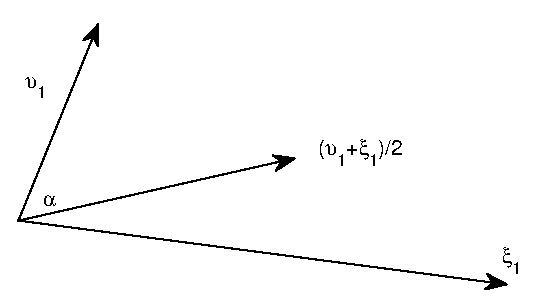
\includegraphics[width=0.65\textwidth]{bending15.eps}
  \end{center}
  \caption{Illustration of the vector of phase.  We assume that the
    bending fiber has two principal orientations, $\bsu_1$ and
    $\bs{\xi}_1$.  If the volume fractions are equal and the
    derivatives of the PDFs at frequency zero are equal, then the
    phase vector will be proportional to the average of these two
    fibers.  Hence, the phase vector will point in the direction of
    bend $(\bsu_1+\bs{\xi}_1)/2$.}
  \label{bending15}
\end{figure}
%%%%%%%%%%%%%%%%%%%%%%%%%%%%%%%%%%%%%%%%%%%%%%%%%%%%%%%%%%%%%%%%%

\subsection{A forking fiber population model}

We consider another model for the asymmetry of the diffusion PDF at
the voxel level that corresponds with a forking structure.  In this
case we again need to adjust Eq.~\eqref{kramermoyal} to that of a
multi-population Eq.~\eqref{mixture},
%\begin{equation}
%  \frac{Z(\q)}{Z(\bld{0})} = \alpha \frac{Z_1(\q)}{Z_1(\bld{0})} +
%  (1-\alpha) \frac{Z_2(\q)}{Z_2(\bld{0})}, 
%\end{equation}
where $Z_1(\q)$ is the fiber population that runs through the entire
voxel and $Z_2(\q)$ is the branching fiber population.  In this
scenario $\cZ_1(\q)\in\bbR$, as this population is symmetric (unless
we wish the fork to have two equal branches, in which case the forking
would be modelled as aggregating three asymmetric branches).  The
phase of the observed signal intensities is given by
\begin{eqnarray}
  \varphi(\q) &=& -\tan^{-1}
  \left(\frac{\Im\{\cZ(\q)\}}{\Re\{\cZ(\q)\}}\right)\\ &=& -\tan^{-1}
  \left(\frac{(1-\alpha)\Im\{\cZ_2(\q)\}}
       {\alpha\cZ_1(\q)+(1-\alpha)\Re\{\cZ_2(\q)\}}\right).
\end{eqnarray}
The concentration of $Z_1(\q)$ and $Z_2(\q)$ will not be uniform on
the sphere in $q$-space.  The most reliable structure in the imaginary
component of the diffusion~PDF will occur when
$|Z_2(\q)|\gg|Z_1(\q)|$.  In this case the phase is changing
perpendicularly to the great circle associated with $Z_2(\q)$, but
there is no phase associated with $Z_1(\q)$.  We plot an example of
this in Fig.~\ref{forking}.  We observe that the phase is more
complicated than in the bending case, and cannot be approximated as
simply linear. The amplitude is still that of a mixture of two PDFs,
while the magnitude of the imaginary part is like a DTI model with two
large eigenvalues and one small. The real part is similar to the
magnitude.

Utilizing the same Taylor series expansion as in the bending case, we
have
\begin{equation}
  \nonumber
  \cA(\q) \approx 1 + \cdots + i \left[(1-\alpha)
  \left(\nabla\cH_{\bs\nu_2}\cA_{2e}(\bld{0})\right)^T\q +
  \cdots\right], 
\end{equation}
and the total phase is given by
\begin{eqnarray}
  \varphi(\q) &\approx& (1-\alpha) \left(\nabla\cH_{\bs\xi_1}
   \cA_{2e}(\bld{0})\right)^T\q\\ 
   &=& (1-\alpha) C_2 \bs\xi_1^T \q
\end{eqnarray}
The orientation of the forking fiber is therefore determined by the
direction of $\varphi(\q)$, or what direction the new fork is going
into, and the magnitude given by the volume fraction and the
derivative of the phase at zero wavenumber.  The sign of the vector
tells us the parity of the forking in a given orientation and provides
additional orientational information.

%%%%%%%%%%%%%%%%%%%%%%%%%%%%%%%%%%%%%%%%%%%%%%%%%%%%%%%%%%%%%%%%%%%%%%
\begin{figure}[tbp]
  \begin{center}
    \begin{tabular}{c|cccc}
      & (i) & (ii) & (iii) & (iv)\\
      \hline
      \\
      (a) & \includegraphics[width=0.2\textwidth]{try460ny.ps} &
      \includegraphics[width=0.2\textwidth]{try160ny.ps} &
      \includegraphics[width=0.2\textwidth]{try260ny.ps} & 
      \includegraphics[width=0.2\textwidth]{try360ny.ps}\\
      \\
      (b) & \includegraphics[width=0.2\textwidth]{try490ny.ps} &
      \includegraphics[width=0.2\textwidth]{try190ny.ps} &
      \includegraphics[width=0.2\textwidth]{try290ny.ps} & 
      \includegraphics[width=0.2\textwidth]{try390ny.ps}
    \end{tabular}
  \end{center}
  \caption{Representations of a simulated forking fiber population for
    a single voxel in $q$-space.  The rows correspond to (a) a
    $60^{\circ}$ bend and (b) a $90^{\circ}$ bend.  The columns
    correspond to (i) the phase, (ii) the absolute value of the real
    part of the complex-valued signal, (iii) the absolute value of the
    imaginary part of the complex-valued signal and (iv) the amplitude
    squared of the complex-valued signal.}
  \label{forking}
\end{figure}
%%%%%%%%%%%%%%%%%%%%%%%%%%%%%%%%%%%%%%%%%%%%%%%%%%%%%%%%%%%%%%%%%%%%%%

\section{Methods}

\subsection{Pre-processing $\bbC$-HARDI data}
\label{preprocessing}

In practice the observations do not take the form of
Eq.~\eqref{qxeqn}.  Instead of a single measurement at each spatial
location and gradient orientation, we have measurements from a number
of coils, that shall here be denoted by $\gamma=1,\dots,N_{\gamma}$
(recall that by coil we actually refer to receiver coils and their
associated electronics).  These observations are all complex-valued,
but have varying sensitivity over space.  In practice, measurements
from all coils must be combined to get an acceptable SNR at the voxel
level in the brain.  All the different coils are subjected to a random
phase-shift common to all the spatial locations, and when treating the
volumes slice-by-slice for fixed superior-inferior coordinates, then a
common movement induced phase may also be modelled.

The nature of phase must be modelled in order to separate
contributions to the $q$-space observations mainly from inter-scan or
intra-scan motion \citep{Aksoyetal2008}), susceptibility effects and
true excess phase due to the observation of asymmetric diffusion~PDFs.
% (such would be the case for example in the case of forking fibers,
% as described above).
Some discussion of motion-induced artifacts causing phase variation
may also be found in; e.g., \citet{Liu2005b}, \citet{Bretthorst} and
\citet{Aksoyetal2008}.

We model the observations at each coil and gradient as a
multiplicative relationship between the true amplitude, a coil
sensitivity effect and an observed phase effect.  These observations
are assumed to have a fixed variance over gradient directions at each
voxel.  We argue that phase due to motion is a large-scale phenomenon,
and estimate this source phase variability using the low-frequency
portion of phase from each coil.  \textbf{We shall discuss the
  susceptibility effects further in section~X}.  This yields an
estimate of the phase at each coil and gradient that needs to be
combined to an estimate at each gradient, based on the stochastic
properties of the raw estimates.  A weighted average is performed
across the coil phases at each gradient, by weighting each phase by
the magnitude of the observation at that coil and gradient
combination.  The details for this entire process is provided in
\ref{preprocessing:step1}.  We also aggregate the magnitudes over the
coils to estimate a single magnitude at each gradient direction.  This
procedure yields an estimator of the complex-valued observations at
each gradient orientation and spatial location whose properties can be
approximated as corresponding to Eq.~\eqref{qxeqn}.
  
\subsection{Least squares estimation of phase}
\label{estimation}

Three important questions are addressed in this section:
\begin{enumerate}
\item Is there remaining (non-Hermitian) mean phase structure at
  $\|\q\|=q$ which cannot be explained by known (artifact-based) causes?
  This is a validation of the pre-processing steps.
\item Is there remaining Hermitian phase structure at $\|\q\|=q$ which
  is statistically significant? 
\item Can we explain the Hermitian structure using a parsimonious
  model, and can we estimate the orientation of the asymmetry?
\end{enumerate}
In order to address these questions we must estimate the structure of
the observed $\bbC$-HARDI data.  With a single estimated amplitude and
phase at each voxel, the parameters of the structure in
Eq.~\eqref{model} may be estimated.  The mean of the real and
imaginary part may be estimated separately, forming the matrices
\begin{eqnarray}
\nonumber
  \bld{A} &=& \begin{pmatrix} 
    \log\left|Z(\q_1)\right| & \cdots & \log\left|Z(\q_L)\right| 
  \end{pmatrix}^T,\\
  \nonumber
  \bld{\Phi} &=& \begin{pmatrix} 
    \phi(\q_{L_0+1}) & \cdots & \phi(\q_L) 
  \end{pmatrix}^T,\\
  %\nonumber
  % \bld{\Phi}_0 &=& \begin{pmatrix} 
  %  \phi(\q_{1}) & \dots & \phi(\q_{L_0}) 
  %\end{pmatrix}^T,\\
  \nonumber
  \bld{P} &=& \begin{pmatrix} 
    1 & -b q_{11}^2 & -b q_{12}^2 & \cdots & -b q_{12} q_{13}\\
    1 & -b q_{21}^2 & -b q_{22}^2 & \cdots & -b q_{22} q_{23}\\
    \vdots & \vdots & \vdots & \ddots & \vdots\\
    1 & -b q_{L1}^2 & -b q_{L2}^2 & \cdots & -b q_{L2} q_{L3}
  \end{pmatrix},\\
  \nonumber
  \bld{R} &=& \begin{pmatrix} 
    1 &  q_{L_0+11} & q_{L_0+12} & q_{L_0+13}\\
    \vdots & \vdots & \vdots & \vdots\\
    1 &  q_{L1} & q_{L2} & q_{L3}
  \end{pmatrix},\\ %\;\bld{r}=\begin{pmatrix} 1\\ \dots \\ 1 \end{pmatrix}\\
  \label{imaginarydir}
  \bs{\alpha} &=& \begin{pmatrix} 
    A_0  & D_{11}^{(2)} & D_{22}^{(2)} & D_{33}^{(2)} & \cdots & D_{23}^{(2)}
  \end{pmatrix}^T,\\
  \bs{\beta} &=& \begin{pmatrix} 
    \Phi_0^{(q)}  & D_1^{(1)} & D_2^{(1)} & D_3^{(1)}
  \end{pmatrix}^T. %\\
  %\bs{\beta}_0 &=& \begin{pmatrix} 
  %  \Phi_0^{(0)}  
  %\end{pmatrix}.
\end{eqnarray}
We then estimate the parameters $\bs{\alpha}$ and $\bs{\beta}$
using the least-squares estimators
\begin{eqnarray}
  \hat{\bs{\alpha}} &=& \left(\bld{P}^T\bld{P}\right)^{-1}
  \bld{P}^T\bld{A},\\
  \hat{\bs{\beta}} &=& \left(\bld{R}^T\bld{R}\right)^{-1}\bld{R}^T
  \bs{\Phi},
\end{eqnarray}
respectively.  We denote the covariance matrix of $\bld{A}$ by
$\bsS_\bld{A}$ and the covariance matrix of $\bs{\Phi}$ as
$\bsS_{\bs{\Phi}}$.  There are no cross correlations between
$\hat{\bs{\alpha}}$ and $\hat{\bs{\beta}}$, as the noise is
approximately complex proper.  The matrices $\bsS_\bld{A}$ and
$\bsS_{\bs{\Phi}}$ are both diagonal with the diagonal entries given
by
\begin{eqnarray*}
  \sigma_{kk}^{(A)} = \var\left\{\log\left|Z(\q_{k+L_0})\right|\right\} &=&
  \frac{\sigma^2}{2\cA^2(\q_{k+L_0})}\\
  &=& \var\left\{\phi(\q_{k+L_0})\right\} = \sigma_{kk}^{(\Phi)},
\end{eqnarray*}
for $k=1,\dots,L-L_0$.  Appealing to the central limit theorem, one
can show that $\hat{\bs{\alpha}}$ and $\hat{\bs{\beta}}$ converge at a
rate of $\sqrt{L}$, and they are asymptotically normally distributed
as $L-L_0\rightarrow\infty$.  This statement is valid unless we
implement a acquisition scheme that samples the sphere densely and in
a very irregular manner.  Following from the theory of least squares
we have that
\begin{eqnarray}
  \nonumber
  \bsS_{\beta} &=& \var\left\{\hat{\bs{\beta}}\right\}\\
  &=& \nonumber
  \var\left\{\left(\bld{R}^T\bld{R}\right)^{-1}\bld{R}^T\bs{\Phi}\right\}\\  
  &=& \left(\bld{R}^T\bld{R}\right)^{-1}\bld{R}^T
  \bsS_\Phi\bld{R} \left(\bld{R}^T\bld{R}\right)^{-1}.
\end{eqnarray}
We can plug in estimators of all these quantities and then obtain
$\wh{\bsS}_{\beta}$.  We have derived estimators for both of
the parameters of interest ($\bs{\alpha}$ and $\bs{\beta}$) and also
and estimate for the variance of $\bs{\beta}$.

Note that the DTI model is estimated from the real part of the
logarithm of the observations; this is equivalent to performing a
regression of the logarithm of the magnitudes, a standard method for
estimating the DTI model \citep{Basser1994}.  We also believe the
model may not be suitable if the voxel corresponds to cortico-spinal
fluid (CSF) or grey matter, as in such cases the distributional
assumptions that make least squares methods suitable are not met. We
propose to remove such voxels from our analysis based on their
fractional anisotropy or mean diffusivity.

% \subsection{Statistical Tests}
% \label{stattest}
% 
% \commentGareth{Not sure if FDR needs to be explained - it's fairly
% standard in neuroimaging} At each voxel a number of statistical
% hypotheses will be tested and, therefore, the $p$-values must be
% adjusted for multiple comparisons.  Our methodology of choice for this
% purpose is the false discovery rate (FDR)
% \citep{Benjamini,gen-laz-nic:thresholding}.  To briefly outline this
% methodology, if we are testing $N$ hypotheses with $p$-values
% $\{p_i\}$, and these are sorted to $\{p_{(i)}\}$ in ascending order,
% then we find the index $i^*$ such that for some chosen significance
% level $p'$
% \begin{equation}
%   p_{(i)} \le \frac{i}{N}p', \quad i=1,\dots,i^*.
% \end{equation}
% Application of FDR results in the first $i^*$ hypotheses being
% rejected, whilst the other $N-i^*$ are not rejected.

\subsubsection{Existence of the remaining phase artifacts}

%We now wish to pursue a number of tests. 
%We start by testing
%whether there are any noticeable susceptibility effects at $b=0$:
%\begin{equation}
%  H_0: \Phi_0^{(0)} = 0, \quad H_1: \Phi_0^{(0)} \neq 0.
%\end{equation}
%Solving the least squares equations gives us:
%\begin{equation}
%  \wh{\Phi}_0^{(0)} = \frac{1}{L_0} \sum_{l=1}^{L_0} \phi(\q_l).
%\end{equation}
%To test the hypothesis we also need a good estimator of $\var\{\wh{\Phi}_0^{(0)}\}$. %For simplicity we take
%\begin{eqnarray}
%\widehat{\var\{\wh{\Phi}_0^{(0)}\}}&=&\sum_{\gamma,j} \frac{1}{n_{\gamma}L_0-1}\left(\theta_{\gamma}(\q_l)-\wh{\Phi}_0^{(0)} %\right)^2,
%\end{eqnarray}
%and then
%\begin{eqnarray}
%T_0&=&\frac{\wh{\Phi}_0^{(0)}-0}{\sqrt{\widehat{\var\{\wh{\Phi}_0^{(0)}\}}}}\sim %N(0,1).
%\end{eqnarray}
%This is a slightly optimistic distributional approximation. The
%reasons %for this are many: firstly, it is harder to remove the
%movement phase for %the $b=0$. If we take a very crude approximation,
%based on only very low-frequency %contributions, then we shall retain
%unpredictable bias terms. If we take %a higher frequency
%approximation, then more often we shall estimate the %phase as $\pm
%\pi$. The normality of all our approximations then falls down. For
%this reason, we re-estimate the variance non-parametrically for both
%%$b=0$ and $b\neq 0$, therefore using the formula above. We do not
%%use the %$b=0$ values when estimating the linear phase term, and so
%%any remaining %biases are less harmful. We remind the reader, that
%%when using Eq.~\eqref{} %to estimate the phase term, it transpires
%%that we cannot use these terms %in any case.

We wish to test the hypothesis that the preprocessing was successful;
this case corresponds to the mean phase over a shell being zero
(assuming discretization effects are negligible).  We formulate the
hypothesis test as
\begin{equation}
  H_0: \Phi_0^{(q)} = 0 \quad \text{versus} \quad H_1: \Phi_0^{(q)}
  \neq 0.
\end{equation}
Solving the least squares equations provides the estimator
$\wh{\Phi}_0^{(q)}=(L-L_0)^{-1}\sum_{l=L_0+1}^{L}\phi(\q_l)$ and the
variance of the estimator is given by
\begin{alignat}{1}
  \var\left\{\wh{\Phi}_0^{(q)}\right\} &= \frac{1}{(L-L_0)^2}
  \sum_{l=L_0+1}^{L} \var\left\{\phi(\q_l)\right\}\\
  &= \frac{1}{(L-L_0)^2} \sum_{l=L_0+1}^{L}
  \frac{\sigma^2}{2\cA^2(\q_l)}.
\end{alignat}
To estimate the components of this expression we need good estimators
of $\sigma^2$ and $\cA^2(\q_l)$.  We use the method of moments
estimator of the observed amplitude square for the latter quantity,
but introduce the robust estimator of
\begin{equation}
  \hat{\sigma}_{\text{MAD}} = \sqrt{2} \; \frac{{\text{median}} 
    \left\{\left|\phi(\q_l) - \phi(\q_{b(l)})\right|
    A(\q_l)\right\}}{0.6745},
\end{equation}
where $b(l)$ is the nearest neighbor of index~$l$.  The factor of
0.6745 is standard to construct an unbiased estimator for Gaussian
data \citep{Hoaglin}.  To obtain a valid test statistic we therefore
take
\begin{equation}
  T_1(q) = \frac{\wh{\Phi}_0^{(q)}\sqrt{2}A(\q_l)}
  {\hat{\sigma}_{\text{MAD}}} \overset{d\,|\,H_0}{=} N(0,1).
\end{equation}
We can therefore (at each voxel) test the hypotheses that
$\Phi_0^{(q)}=0$; by calculating an observed value of $T_1$ and
comparing this to the standard Gaussian distribution.  If the average
phase is non-zero, then this is indicative of either insufficient
removal of phase induced by movement, or remaining susceptibility
effects.  In either case, the Hermitian structure is not in this case
interpretable, as deviating from a non-zero mean.  These voxels should
be removed from further analysis.

\subsubsection{Existence of Hermitian phase structure}

The second test corresponds to testing whether the Hermitian structure
is non-negligible or:
\begin{equation}
  H_0: \bld{d}^{(\im)} = \bld{0} \quad \text{versus} \quad 
  H_1: \bld{d}^{(\im)} \neq \bld{0}. 
\end{equation}
This test is formulating the question, is there any asymmetry in the
diffusion~PDF, or is this wholly symmetric?  Define
$\bF=\text{diag}\left(0,\,1,\,1,\,1\right)$, and then the Wald
statistic for this problem is given by
\begin{equation}
  T_2 = \left(\bF\hat{\bs{\beta}}\right)^T
  \left(\bF\wh{\bsS}_{\beta}\bF^T\right)^{-1}
  \bF\hat{\bs{\beta}} \overset{d\,|\,H_0}{=} \chi^2_3.
\end{equation}
This then provides us with the means to test for Hermitian structure
in the phase.  The information of the $\bld{d}^{(\im)}$ vector is
important for two reasons: it provides us with a method of detecting
Hermitian structure present in the data and we may estimate the
orientation of that direction and so both the magnitude and the
directionality of this object is of interest.

\subsubsection{Existence of linear phase structure}

Finally, having established that no artificial or random phase shifts
remain, and that Hermitian structure can be found in the data, we may
wish to try to estimate this structure by a moderate number of
parameters.  We saw from our previous arguments that bending fibers
have near linear phase, whilst forking/fanning fibers have more
complicated phase.  We therefore fit a linear term to the phase, to
capture the main hermitian structure.  If the structure is consistent
with bending, then the linear terms should capture most of the
structure in the phase.  In this case $R^2$ (the coefficient of
determination) from fitting the linear phase model should take a value
near one.  By calculating $R^2$ we may determine how near linear the
phase is.

We define $R^2$ to be the fraction of energy explained by the linear
term
\begin{equation}
  R^2 = \frac{\sum_{l=1}^{L-L_0} \left(\hat{d}_1^{(q)}q_{L_0+l,1}
    + \hat{d}_2^{(q)}q_{L_0+l,2} + \hat{d}_3^{(q)}q_{L_0+l,3}\right)^2}
  {\sum_{l=1}^{L-L_0}\phi_l^2}.
\end{equation}
Note that when estimating $\bld{d}$ we also estimate the $\Phi_0(q)$
term, and so no non-zero mean phase terms will bias our estimation of
$\bld{d}$ (it is bad practice to estimate the linear term before the
main effect).  Recall that we want to keep a potentially non-zero main
effect in the model (insufficient phase removal) and then see what
fraction of energy is explained by the linear (Hermitian) terms.  A
Taylor series expansion may justify this (\textit{cf.}
Eq.~\eqref{taylor:phase2}), and see also the plots in
Figs.~\ref{bending} and~\ref{forking}.  Since it is true that
$\sum_j\q_j\approx\bld{0}$ it however makes little difference whether
one includes a mean term or not when estimating the linear terms.
Note that unlike DTI we must sample the entire sphere instead of a
half-sphere to estimate this effect.

\subsection{Model comparison}

As a real-valued method of comparison we shall fit three possible
models, namely the isotropic model of
\begin{equation}\label{isotropic}
  \cA(\bq_l) = \cA(q), \quad l=L_0+1, \dots, L,
\end{equation}
the single tensor model of
\begin{equation}\label{singletensor}
  \cA(\bq_l) = \exp\left\{-\frac{1}{2}\q^T\bD^{(\re)}\q\right\}, 
\end{equation}
$l=1,\dots,L$, as well as the two tensor model of 
\begin{equation}\label{doubletensor}
  \cA(\bq_l) = \frac{1}{2}\exp\left\{-\frac{1}{2} \q^T \bD^{(\re)}_1
  \q\right\} + \frac{1}{2}\exp\left\{-\frac{1}{2} \q^T \bD^{(\re)}_2
  \q\right\},
\end{equation}
$l=L_0+1,\dots,L$.  Note that we have in the latter case enforced
equal weighting between fibers of a half.  This is to ensure model
identifiability.  Basically, if we only collect measurements at $b=0$
and a single shell we can receive the same value for
$a_1\exp\{-{\q}^T\bD^{(\re)}_1{\q}/2\}$ by equivalently changing the
scaling of $\bD^{(\re)}_1$ or the volume fraction.  To ensure
identifiability we either need to fix the trace of the diffusion
matrices or the volume fractions.

For simplicity we first normalize the measurements by the following
rule
\begin{eqnarray}
  \ol{A}(\bld{0}) &=& \frac{1}{L_0}\sum_{l=1}^{L_0}
  \sum_{\gamma} A_{\gamma}(\q_l),\quad 
  \wt{A}(\q_l) = \frac{\sum_\gamma A_\gamma(\q_l)}{\ol{A}(\bld{0})}.
\end{eqnarray}
This ensures the PDF estimate has been normalized. To produce
estimated fitted models we would use the objective function:
\begin{equation}
  \hat{\bs{\theta}} = \argmin \sum_{l=L_0+1}^L \left[\wt{A}(\q_l) -
  \cA(\bq_l)\right]^2,
\end{equation}
where $\hat{\bs{\theta}}=()$ \textbf{[WHAT is $\hat{\bs{\theta}}$]} and
$\cA(\bq_l)$ is given by Eqs.~\eqref{isotropic}, \eqref{singletensor}
or~\eqref{doubletensor}.  This however does not allow us to easily
chose between the models of Eqs.~\eqref{isotropic},
\eqref{singletensor} or~\eqref{doubletensor}.  It is natural that
Eq.~\eqref{doubletensor} fits the data better than
Eq.~\eqref{isotropic} because it has more parameters.  We denote the
number of parameters in any one model by $p$. We therefore account for
``learning of the noise'' by using a model choice procedure.  We here
apply the Bayesian Information Criterion (BIC) \citep{Schwarz},
% as this is known to penalize overfitting better than Aikake's
% Information Criterion AIC 
and define the new optimization problem of
\begin{equation}\label{eq:BIC}
  \left[\hat{\bs{\theta}},\hat{p}\right] = \argmin \left\{(L-L_0)
  \log\left[\frac{1}{L-L_0}\sum_{l=L_0+1}^L
  \left(\wt{A}(\q_l)-\cA(\bq_l)\right)^2\right] + p\log[L-L_0]
  \right\}.
\end{equation}
This will permit us to both chose the model and estimate the
parameters of the best fitting model.  We reiterate that bending
fibers are more likely to be seen as single-tensor models, and forking
fibers as mixture models.  \commentSofia{We seem to underutilize the
simulations. Brandon didn't like the extra plots, so I removed them,
but maybe we should use a table or something?}

\subsection{Clinical data acquisition}

\textit{In vivo} data were acquired on a single healthy male
volunteer, who gave informed consent according to local policies,
using a GE Signa HDx system (General Electric, Waukshua, WI, USA),
with actively shielded magnetic field gradients (maximum amplitude
$40\;\text{mT/m}^{-1}$).  The body coil was used for RF transmission,
and an eight-channel head coil for signal reception.  No parallel
imaging speedup method was applied in order to simplify data
processing.  Each volume was acquired using a ``peripherally gated''
% [SOFIA I THINK THIS IS THE DATASET YOU USED IN THE END? (Series 0005). IF 
% NOT, (i.e. if you used 0004, which was ungated) JUST DELETE THESE LAST TWO 
% WORDS] 
multi-slice singly refocused spin echo EPI sequence, with parameters
optimised for precise measurement of the diffusion tensor in
parenchyma, with isotropic ($2.5{\times}2.5{\times}2.5\;\text{mm}$)
voxels and a $128{\times}128$ in-plane matrix.  Because of scanner
limitations, only 19 slices were acquired per volume.  Hence, an
interslice gap of $2.5\;\text{mm}$ was used to ensure most of the
brain was surveyed.  Repetition time was set to 5 R-R intervals, 
% [IF YOU USED THE GATED DATA, WHICH I THINK YOU DID]
% $4000\;\text{ms}$,
% [IF YOU USED THE NON-GATED DATA]
and the echo time was extended to $150\;\text{ms}$ to allow full echo
data to be collected and thus avoid the complication of the homodyne
reconstruction which would otherwise be necessary.  

Based on the recommendations of \citet{DKJones99},
% (Jones DK, Williams SCR, Gasston D, Horsfield MA, Simmons A, Howard
% R. Isotropic resolution diffusion tensor imaging with whole brain
% acquisition in a clinically acceptable time. Hum Brain Mapp 2002;
% 15: 216-230)
the maximum diffusion weighting was $1300\;\text{s/mm}^{-2}$, and at
each slice location, two images were acquired with no diffusion
gradients applied, together with 26 diffusion-weighted images in which
gradient directions were uniformly distributed in space.  As with the
number of slice locations, choices for these parameters were severely
constrained by scanner limitations.  For each volume (i.e., each set
of 19 slice locations), complex data was stored as separate real and
imaginary images for each of the eight receive coils, along with a
coil-combined (magnitude) image automatically created by the scanner.
GE's ``gradwarp'' processing (which attempts to correct for minor
image distortions due to imaging gradient non-linearities) was
disabled for all images.

The coil-combined magnitude images were corrected for the effects of
eddy-current induced distortion and subject motion using in-house
software.  For each data set, a two-stage registration process was
used.  First, the diffusion-weighted volumes were co-registered
together (using the mean diffusion weighted volume as reference) with
a 12-parameter 3D affine transformation.  The non-diffusion weighted
volumes were similarly co-registered, but with a six-parameter rigid
body transformation.  The co-registered non-diffusion weighted volumes
were then registered to the co-registered diffusion-weighted volumes
by another six-parameter rigid body transformation.  Each registration
step used the FLIRT routine, part of FSL
\citep{jen-smi:global,smi-etal:FSL}.  The transformations determined
by this process were then applied to the set of 16 corresponding
images from the complex-valued data (i.e., real and imaginary images
for each of eight coils).

\subsection{Simulations}
\label{methods-simulations}

The simulation of fiber population structures involves the combination
of Gaussian and non-Gaussian models as diffusion PDFs.  We model this
structure directly in $q$-space.  As a starting point, we provide the
standard Gaussian diffusion tensor model
\begin{equation}\label{GaussianDTI}
  \text{G}(\q;\bsL,\bld{V}) = \exp\left(-\lambda_1\langle\bsu_1,
  \q\rangle^2-\lambda_2 \langle\bsu_2,
  \q\rangle^2-\lambda_3\langle\bsu_3, \q\rangle^2\right),
\end{equation} 
where $\bsL=\text{diag}(\lambda_1,\lambda_2,\lambda_3)$ is the
diagonal matrix of eigenvalues and $\bld{V}=\{\bsu_k\}_k$ is the
matrix of eigenvectors.  The half-Gaussian diffusion model is given by
\begin{eqnarray}
  \nonumber
  \text{HG}(\q;\bsL,\bld{V}) &=&
  \exp\left(-\lambda_2\langle\bsu_2,\q\rangle^2\right)
  \exp\left(-\lambda_3\langle\bsu_3,\q\rangle^2\right)\\
  & & \times\left[\exp\left(-\lambda_1\langle\bsu_1,\q\rangle^2\right)
  - i \frac{2}{\sqrt{\pi}} D\left(\sqrt{\lambda_1}\langle \bsu_1, \q
  \rangle\right)\right],
  \label{Dawson}
\end{eqnarray}
where $D(\cdot)$ is the Dawson function \citep{abra}.  The phase of
the half-Gaussian diffusion model is given by
\begin{eqnarray}\label{angle:halfG}
  \varphi^{(\text{HG})}(\q) &=& -\tan^{-1}
  \left(\frac{-\frac{2}{\sqrt{\pi}} D\left(\sqrt{\lambda_1}
  \langle\bsu_1, \q \rangle\right)} {\exp\left(-\lambda_1\langle\bsu_1, \q\rangle^2\right)}\right)\\
  &\approx & \frac{2}{\sqrt{\pi}}\sqrt{\lambda_1}\langle \bsu_1, \q
  \rangle + \cdots.
\end{eqnarray}
We provide a plot of the true phase, and its linear approximation, in
Fig.~\ref{phaseplot} for a number of $\lambda_1$ namely
$\lambda_1=0.54$ (dash-dotted) $\lambda=2.72$ (solid) and
$\lambda=13.60$ (dotted).  The linear phase approximation, represented
by the thick line for each line style and $\lambda_1$ value, appears
to be reasonable for the half-Gaussian diffusion model as long as $q$
does not become too large, in absolute value.

%%%%%%%%%%%%%%%%%%%%%%%%%%%%%%%%%%%%%%%%%%%%%%%%%%%%%%%%%%%%%%%%%%%%%%
\begin{figure}[!htbp]
  \begin{center}
    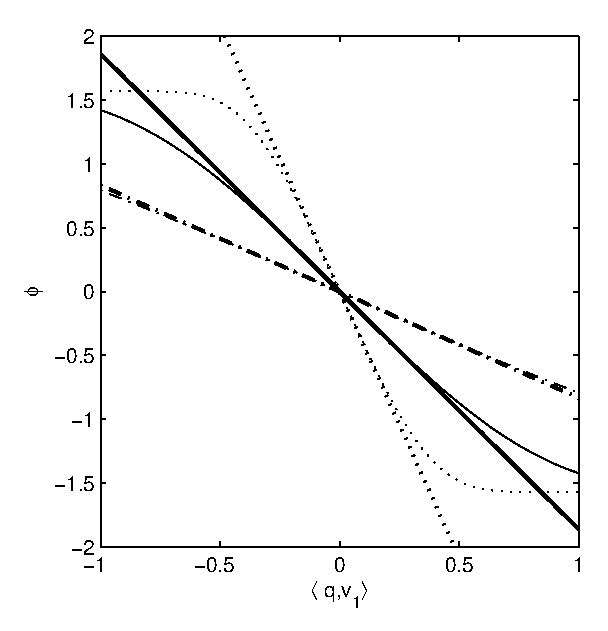
\includegraphics[width=0.5\textwidth]{phase1.eps}
  \end{center}
  \caption{A plot of the phase of the half-Gaussian diffusion model as
    a function of the principle eigenvalue $\lambda_1$.  The
    approximation given by Eq.~\eqref{angle:halfG} is represented as
    the thick line, for each line style.  The value of $\lambda_1$ is
    indicated by the line style, namely $\lambda_1=0.54$ (dash-dotted)
    $\lambda=2.72$ (solid) and $\lambda=13.60$ (dotted).}
  \label{phaseplot}
\end{figure}
%%%%%%%%%%%%%%%%%%%%%%%%%%%%%%%%%%%%%%%%%%%%%%%%%%%%%%%%%%%%%%%%%%%%%%

We propose five different fiber population structures in order to
investigate the typical characteristics of diffusion PDFs discussed
previously.  Table~\ref{simulationtable} provides a summary of these
models, where $\bsL^{(1)}=0.04\cdot{\text{diag}}(17\times4,8,8)$,
$\bsL^{(2)}=0.04\cdot{\text{diag}}(84/3,84/3,84/3)$.  The orientation
of the first diffusion~PDFs is chosen randomly, and is given by the
basis $\bld{V}$, while the orientation of the second PDF is rotated by
an angle of $\theta$ in the third axis ($q_3$).
% The notation $\text{TPD}(\q_l)$ is a truncated prolate diffusion
% process, $\text{PD}(\q_l)$ is a prolate diffusion process,
% $\text{ID}(\q_l)$ is an isotropic diffusion process,
% $\text{FD}(\q_l)$ is a forking diffusion process and
% $\text{BD}(\q_l)$ is a bending diffusion process.

%%%%%%%%%%%%%%%%%%%%%%%%%%%%%%%%%%%%%%%%%%%%%%%%%%%%%%%%%%%%%%%%%%%%%%
\begin{table}[tbp]
  \caption{Summary of fiber population structure models used in the
    simulations.  The functions $\text{G}(\q_l)$ and $\text{HG}(\q_l)$
    are defined in Eqs.~\eqref{GaussianDTI} and \eqref{Dawson},
    respectively.}
  \label{simulationtable}
  \begin{center}
    \begin{tabular}{lcc}
      \hline
      \textbf{Name} & \textbf{Notation} & \textbf{Function}\\
      \hline
      Truncated Prolate Diffusion Process & $\text{TPD}(\q_l)$ &
      $\text{HG}(\q_l;\bsL^{(1)},\bld{V})$\\
      Prolate Diffusion Process & $\text{PD}(\q_l)$ &
      $\text{G}(\q_l;\bsL^{(1)},\bld{V})$\\
      Isotropic Diffusion Process & $\text{ID}(\q_l)$ &
      $\text{HG}(\q_l;\bsL^{(2)},\bld{V})$\\
      Forking Diffusion Process & $\text{FD}(\q_l)$ &
      $\frac{2}{3}\text{G}(\q_l;\bsL^{(1)},\bld{V}) +
      \frac{1}{3}\text{HG}(\q_l;\bsL^{(1)},R_\theta\bld{V})$\\
      Bending Diffusion Process & $\text{BD}(\q_l)$ &
      $\frac{1}{2}\text{HG}(\q_l;\bsL^{(1)},\bld{V}) +
      \frac{1}{2}\text{HG}(\q_l;\bsL^{(1)},R_\theta\bld{V})$\\
      \hline
    \end{tabular}
  \end{center}
\end{table}
%%%%%%%%%%%%%%%%%%%%%%%%%%%%%%%%%%%%%%%%%%%%%%%%%%%%%%%%%%%%%%%%%%%%%%

\section{Results}
\label{results}

\subsection{Simulated data} % see the script testcomplex2.m

We simulate diffusion~PDFs following \citet{Alexander2005} in the
class of diffusion parameters, but adjust the PDFs to match our choice
of $b=1300$.  Both in the simulation studies and the clinical data
acquisition we use a set of gradients determined using the method of
\citet{DKJones99}.  The signal-plus-noise model is given by
\begin{eqnarray}
  Z(\q_l) &=& \cZ^{(k)}(\q_l) + \sigma\epsilon_l + i\sigma\eta_l\\
  \cZ(\q_l) &=& \cA(\q_l) \exp\left(-i\varphi^{(k)}(\q_l)\right),
\end{eqnarray}
where $\cZ(\cdot)$ is one of the fiber population structure models in
Section~\ref{methods-simulations}, $\epsilon_l$ and $\eta_l$ are
independent realizations from a Gaussian distribution with equal
standard deviations of $\text{TPD}(\bld{0})/20$.  We randomize each
trial over $\{\bsu_1\}$ to avoid consistent directional biases,
selecting two perpendicular vectors to this eigenvector and force the
error standard deviation to be $\sigma=1/20$.  We also rotate the
second basis $\{\bs{\xi}_j\}_j$ with respect to the first by $\theta$
in the $q_3$ axis, where $\theta\in\{\pi/3,\pi/2\}$.  Because $\bsu_1$
has a random orientation, no consistent orientational biases are
accrued by this procedure.

%%%%%%%%%%%%%%%%%%%%%%%%%%%%%%%%%%%%%%%%%%%%%%%%%%%%%%%%%%%%%%%%%%%%%%
\begin{figure}[tbp]
  \begin{center}
    \begin{minipage}[]{0.45\textwidth}
      \centering
      \textbf{Sparse Sampling}\\
      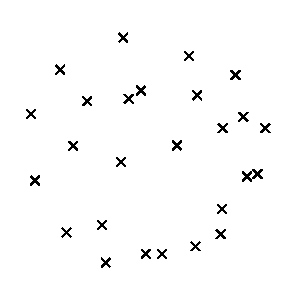
\includegraphics[width=\textwidth]{cloudlowden.eps}
    \end{minipage}
    \begin{minipage}[]{0.45\textwidth}
      \centering
      \textbf{Dense Sampling}\\
      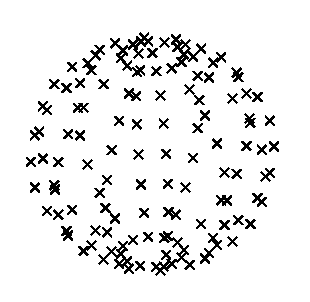
\includegraphics[width=\textwidth]{cloudhighden.eps}
    \end{minipage}
  \end{center}
  \caption{Directionoal sampling regimes for the simulation study:
    26~gradient directions (\textit{sparse sampling}) used in the
    clinical acquisition \citep{DKJones99} and a regular sampling of
    the sphere with 133~gradient directions (\textit{dense
      sampling}).}
  \label{fig:sampling}
\end{figure}
%%%%%%%%%%%%%%%%%%%%%%%%%%%%%%%%%%%%%%%%%%%%%%%%%%%%%%%%%%%%%%%%%%%%%%

%%%%%%%%%%%%%%%%%%%%%%%%%%%%%%%%%%%%%%%%%%%%%%%%%%%%%%%%%%%%%%%%%%%%%%
\begin{figure}[tbp]
  \begin{center}
    \begin{minipage}[]{0.45\textwidth}
      \centering
      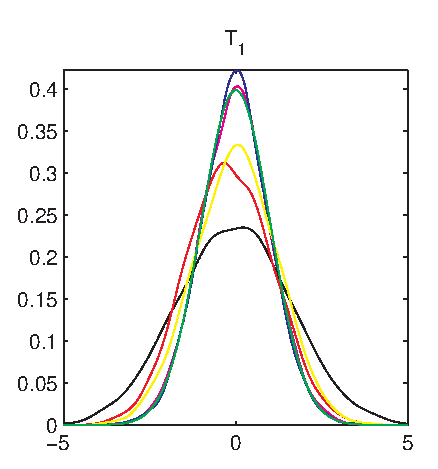
\includegraphics[width=\textwidth]{mrmcomplex14ny.eps}
      (a)
    \end{minipage}
    \begin{minipage}[]{0.45\textwidth}
      \centering
      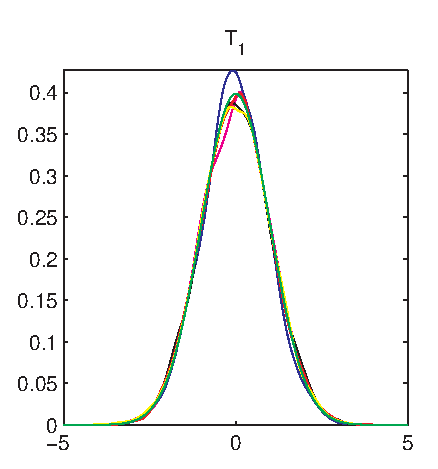
\includegraphics[width=\textwidth]{mrmcomplex14nyhighden.eps}
      (b)
    \end{minipage}
    \begin{minipage}[]{0.45\textwidth}
      \centering
      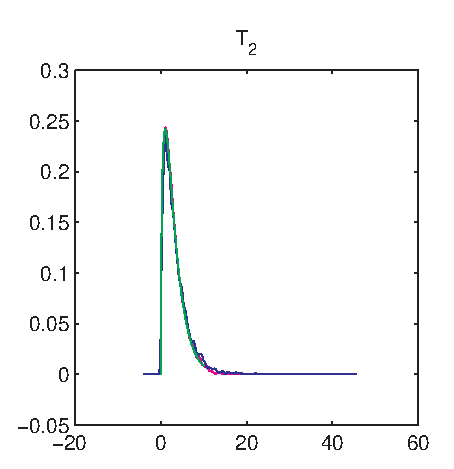
\includegraphics[width=\textwidth]{mrmcomplex15ny.eps}
      (c)
    \end{minipage}
    \begin{minipage}[]{0.45\textwidth}
      \centering
      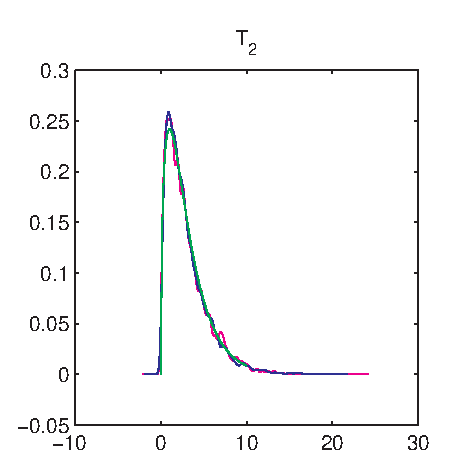
\includegraphics[width=\textwidth]{mrmcomplex15nyhighden.eps}
      (d)
    \end{minipage}
  \end{center}
  \caption{Test statistics $T_1$ and $T_2$ from simulations under two
    $q$-space sampling schemes.  \textbf{(a,c)} use the \textit{sparse
      sampling} scheme and \textbf{(b,d)} use the \textit{dense
      sampling}) scheme.  The color coding is green for the
    theoretical diffusion~PDF, maroon for the isotropic, red for the
    half-Gaussian, yellow for the bending fibre, black for the
    branching and blue for the the usual DTI prolate model.
    \textbf{[Maybe better to have a legend for the colors?  Thicker
        lines?]}}
  \label{fig:T1T2}
\end{figure}
%%%%%%%%%%%%%%%%%%%%%%%%%%%%%%%%%%%%%%%%%%%%%%%%%%%%%%%%%%%%%%%%%%%%%%

We simulate the artificial DW-MRI acquisitions 5000 times, and apply
parametric methods to calculate summary statistics, as outlined in the
previous section.  Fig.~\ref{fig:sampling} displays the directions
associated with the sparse sampling scheme (26~directions) and dense
sampling scheme (133~directions) on the sphere.  First, we look at the
behavior of the test statistics, the null average phase $T_1$ and the
Wald statistic$T_2$, under the diffusion models in
Table~\ref{simulationtable}.
% Fig.~\ref{fig:T1T2} shows the two statistics of interest $T_1$ and
% $T_2$, and Fig.~\ref{fig-1} shows the quantitative descriptions of
% the complex structure.
When compared with their theoretical distributions, a $N(0,1)$ for the
$T_1$ statistic and a $\chi^2_3$ for the $T_2$ statistic,
Fig.~\ref{fig:T1T2} shows the consistent performance of our
statistics.  The simulated data should have zero average phase and no
Hermitian phase and this is confirmed by the fact that the empirical
distributions for each statistic closely match the theoretical
distribution.  However, we acknowledge the fact that the theoretical
distribtion for null average phase is more difficult to achieve for
certain diffusion models using a sparse sampling of directions over
the sphere.

%%%%%%%%%%%%%%%%%%%%%%%%%%%%%%%%%%%%%%%%%%%%%%%%%%%%%%%%%%%%%%%%%%%%%%
\begin{figure}[tbp]
  \begin{center}
    \begin{minipage}[]{0.45\textwidth}
      \centering
      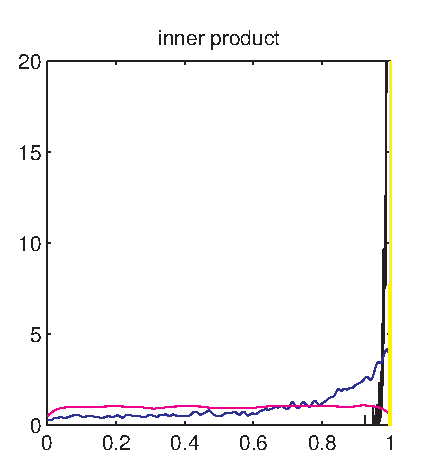
\includegraphics[width=\textwidth]{inner_product.eps}
      \textbf{(a)}
    \end{minipage}
    \begin{minipage}[]{0.45\textwidth}
      \centering
      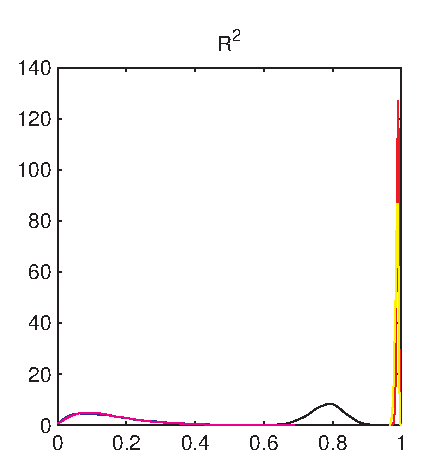
\includegraphics[width=\textwidth]{R2.eps}
      \textbf{(b)}
    \end{minipage}
  \end{center}
  \caption{Estimating the linear phase term under the sparse sampling
    scheme: \textbf{(a)} the norm of $\bd^{(\text{im})}$ and
    \textbf{(b)} the coefficient of determination $R^2$ from the
    linear regression.  The two real-valued diffusions (prolate, blue)
    and (isotropic, purple), forking fibre (black), a single
    asymmetric diffusion (red), or bending fibre (yellow).}
  \label{fig-1} 
\end{figure}
%%%%%%%%%%%%%%%%%%%%%%%%%%%%%%%%%%%%%%%%%%%%%%%%%%%%%%%%%%%%%%%%%%%%%%

Additional statistics of interest when estimating the linear phase
structure are the norm of the imaginary vector $\bd^{(\text{im})}$ and
the coefficient of determination $R^2$.  In Fig.~\ref{fig-1} it is
apparent that the asymmetric diffusion~PDFs are clearly distinguished
from the symmetric PDFs, by observing different values of the Wald
statistic \textbf{[is this correct?!?]} and that the imaginary
structure is described by the varying value of the norm of the
imaginary vector $\bd^{(\text{im})}$.  \textbf{[WHAT?!?]}

We would like to distinguish between simple forms of the phase, as
would be typical for bending, and more complex forms that cannot be
characterised by a linear phase, as in forking, compare with the plots
in Figs.~\ref{bending}--\ref{forking}.  If one looks at the
Figs.~\ref{bending}(a,i) and~\ref{bending}(b,i), and compares them to
Figs.~\ref{forking}(a,i) and~\ref{forking}(b,i), it is apparent that
the main structure of Figs.~\ref{bending}(a,i) and~\ref{bending}(b,i)
may be described as linear, but Figs.~\ref{forking}(a,i)
and~\ref{forking}(b,i) are clearly not linear.
Fig.~\ref{forking}(a,i) exhibits additional asymmetry, while
Fig.~\ref{forking}(b,i) has the additional double maxima.  Such
empirical observations are born out by the distributional results in
Fig.~\ref{fig-1}(b).  \textbf{[More discussion about Figure~6!!!]}

\subsection{Clinical data}

%%%%%%%%%%%%%%%%%%%%%%%%%%%%%%%%%%%%%%%%%%%%%%%%%%%%%%%%%%%%%%%%%%%%%%
\begin{figure}[p]
  \begin{center}
    \begin{minipage}[]{.42\textwidth}
      \centering
      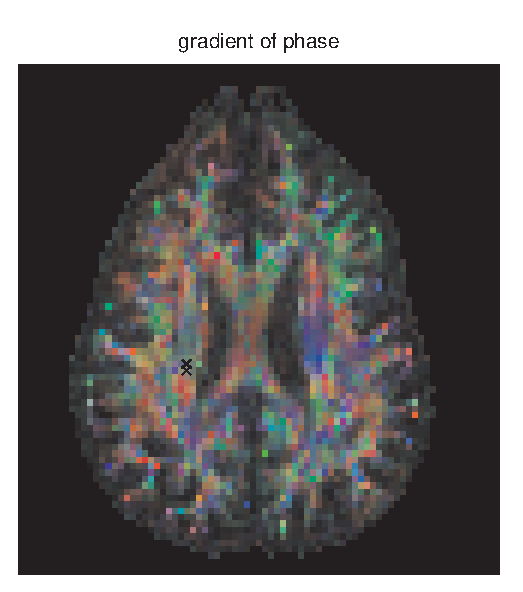
\includegraphics[width=\textwidth]{gradphasebu.eps}
      (a)
      \end{minipage}
      \begin{minipage}[]{.42\textwidth}
      \centering
      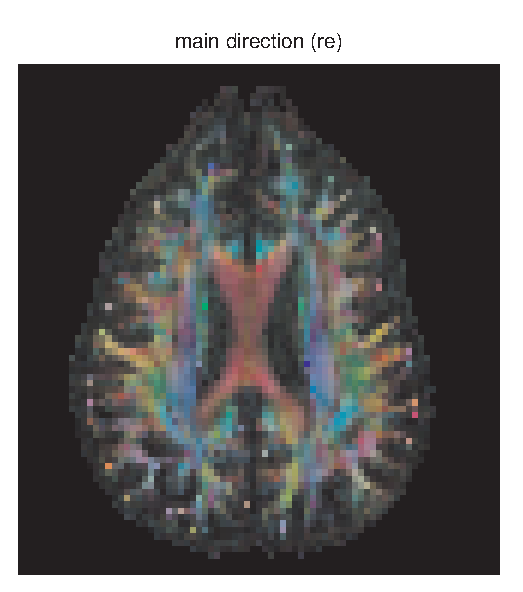
\includegraphics[width=\textwidth]{maindirecreal.eps}
      (b)
      \end{minipage}
      \begin{minipage}[]{.42\textwidth}
      \centering
       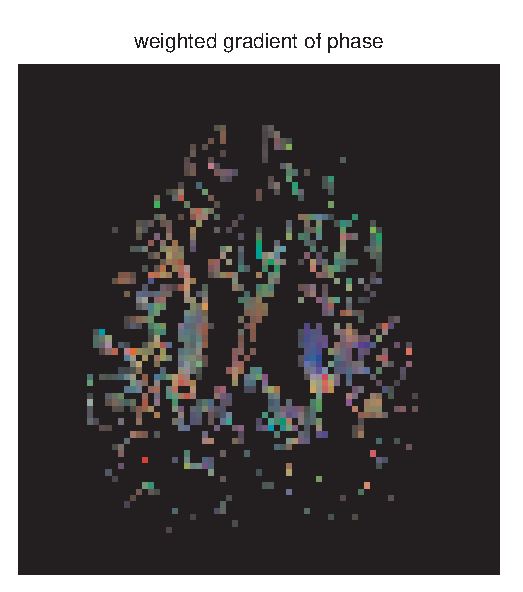
\includegraphics[width=\textwidth]{1gradphase55b.eps}
       (c)
      \end{minipage}
      \begin{minipage}[]{.42\textwidth}
      \centering
      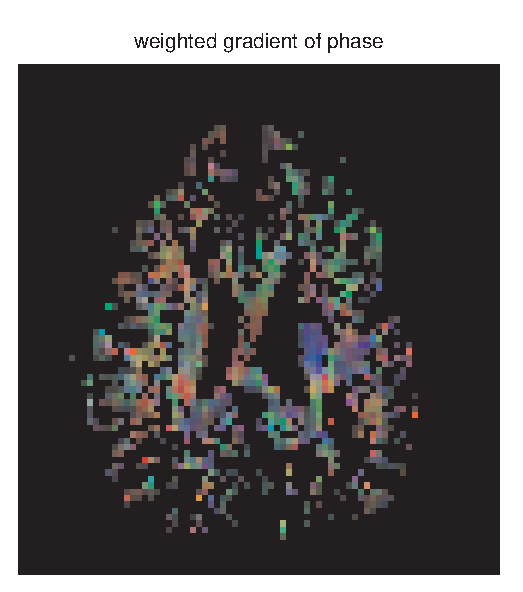
\includegraphics[width=\textwidth]{1gradphase55d.eps}
      (d)
    \end{minipage}
  \end{center}
  \caption{Estimated orientations from {\em in vivo} data using the
    (a) gradient of the phase and (b) the dominant direction of the
    amplitude, (c) and (d) showing only directions that may be
    considered statistically significant (see the text for
    details). This is slice 10.}
  \label{fig1} 
\end{figure}
%%%%%%%%%%%%%%%%%%%%%%%%%%%%%%%%%%%%%%%%%%%%%%%%%%%%%%%%%%%%%%%%%%%%%%

%%%%%%%%%%%%%%%%%%%%%%%%%%%%%%%%%%%%%%%%%%%%%%%%%%%%%%%%%%%%%%%%%%%%%%
\begin{figure}[p]
  \begin{center}
   \begin{minipage}[]{.42\textwidth}
      \centering
      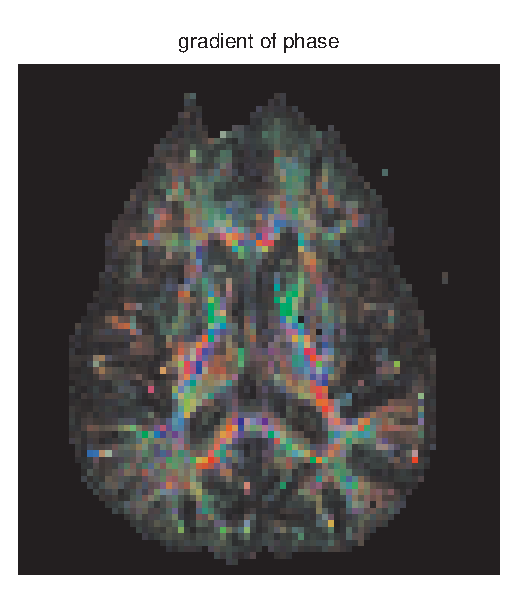
\includegraphics[width=\textwidth]{gradphase55a.eps}
      (a)
      \end{minipage}
       \begin{minipage}[]{.42\textwidth}
      \centering
      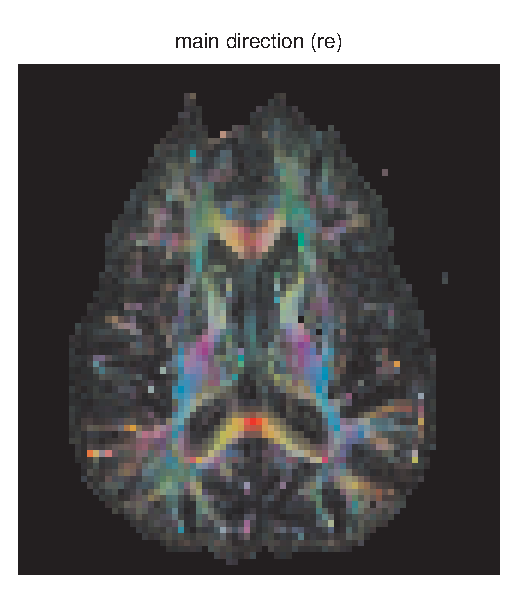
\includegraphics[width=\textwidth]{tensdir55.eps}
        (b)
      \end{minipage}\\
       \begin{minipage}[]{.42\textwidth}
      \centering
       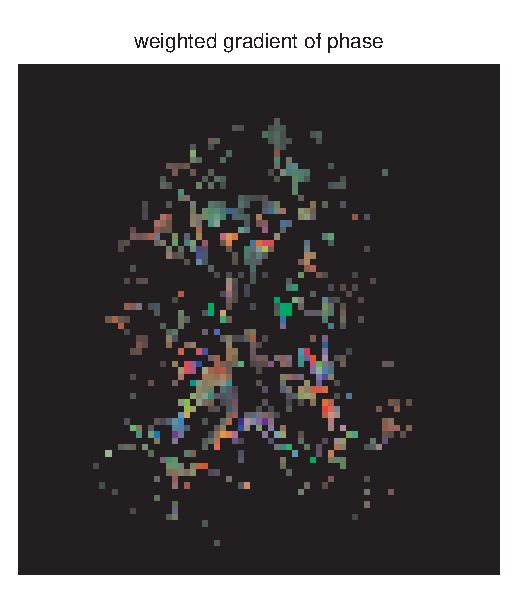
\includegraphics[width=\textwidth]{gradphase55b.eps}
         (c)
      \end{minipage}
        \begin{minipage}[]{.42\textwidth}
      \centering
      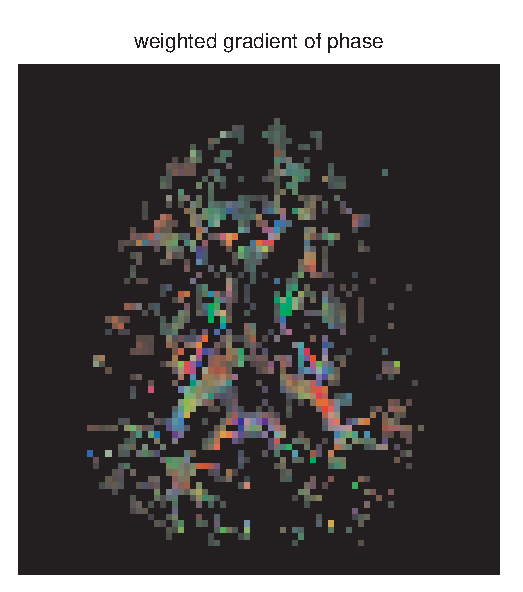
\includegraphics[width=\textwidth]{gradphase55d.eps}
      (d)
    \end{minipage}
  \end{center}
  \caption{Estimated orientations from {\em in vivo} data using the
    (a) gradient of the phase and (b) the dominant direction of the
    amplitude, (c) and (d) showing only directions that may be
    considered statistically significant (see the text for
    details). This is slice 7.}
  \label{fig1b} 
\end{figure}
%%%%%%%%%%%%%%%%%%%%%%%%%%%%%%%%%%%%%%%%%%%%%%%%%%%%%%%%%%%%%%%%%%%%%%

%%%%%%%%%%%%%%%%%%%%%%%%%%%%%%%%%%%%%%%%%%%%%%%%%%%%%%%%%%%%%%%%%%%%%%
\begin{figure}[p]
  \begin{center}
      \begin{minipage}[]{0.42\textwidth}
      \centering
      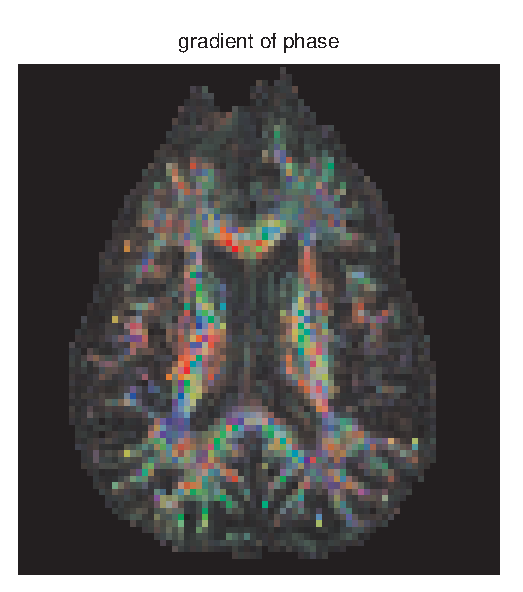
\includegraphics[width=\textwidth]{gradphase55any.eps}
       (a)
    \end{minipage}
      \begin{minipage}[]{0.42\textwidth}
      \centering
      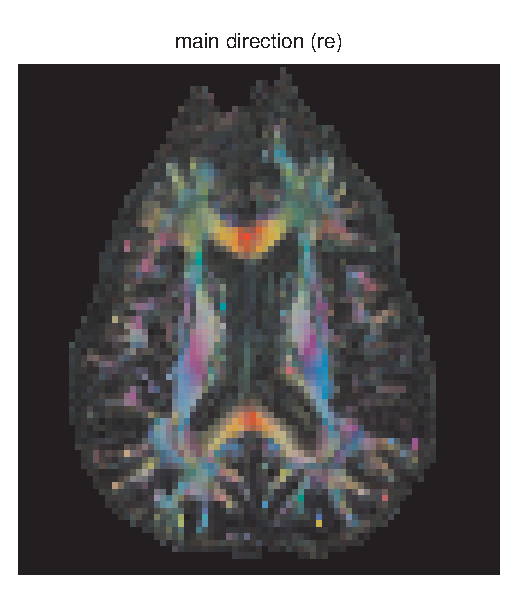
\includegraphics[width=\textwidth]{tensdir55ny.eps}
       (b)
    \end{minipage}
      \begin{minipage}[]{0.42\textwidth}
      \centering
       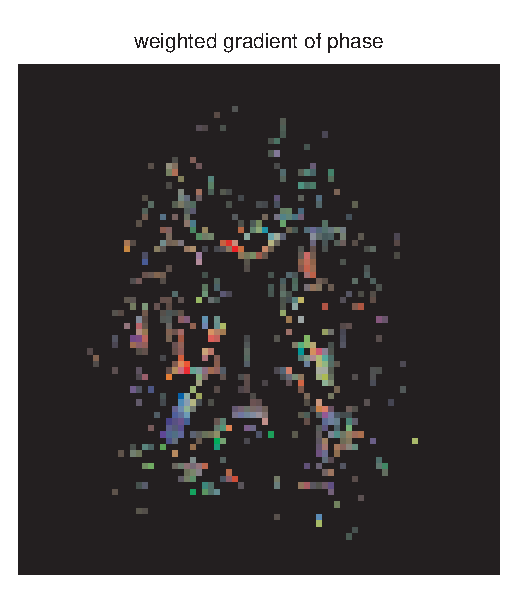
\includegraphics[width=\textwidth]{gradphase55bny.eps}
        (c)
    \end{minipage}
      \begin{minipage}[]{0.42\textwidth}
      \centering
      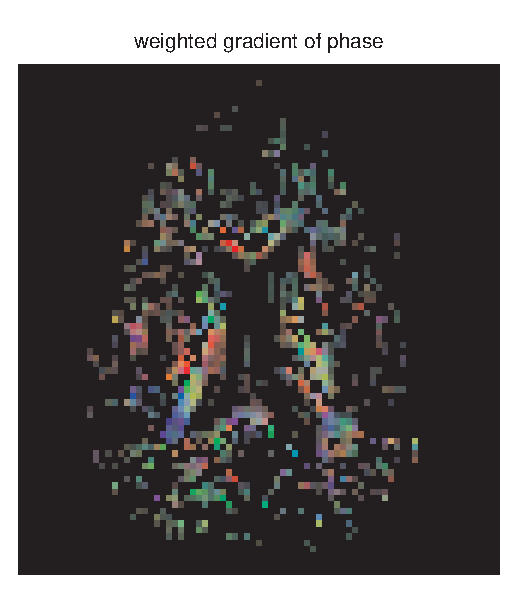
\includegraphics[width=\textwidth]{gradphase55dny.eps}
      (d)
    \end{minipage}
  \end{center}
  \caption{Estimated orientations from \textit{in vivo} data using the
    (a) gradient of the phase and (b) the dominant direction of the
    amplitude, (c) and (d) showing only voxels where these may be
    considered statistically significant (see the text for details).}
  \label{fig1c} 
\end{figure}
%%%%%%%%%%%%%%%%%%%%%%%%%%%%%%%%%%%%%%%%%%%%%%%%%%%%%%%%%%%%%%%%%%%%%%

%%%%%%%%%%%%%%%%%%%%%%%%%%%%%%%%%%%%%%%%%%%%%%%%%%%%%%%%%%%%%%%%%%%%%%
\begin{figure}[p]
  \begin{center}
    \begin{minipage}[]{.30\textwidth}
      \centering
      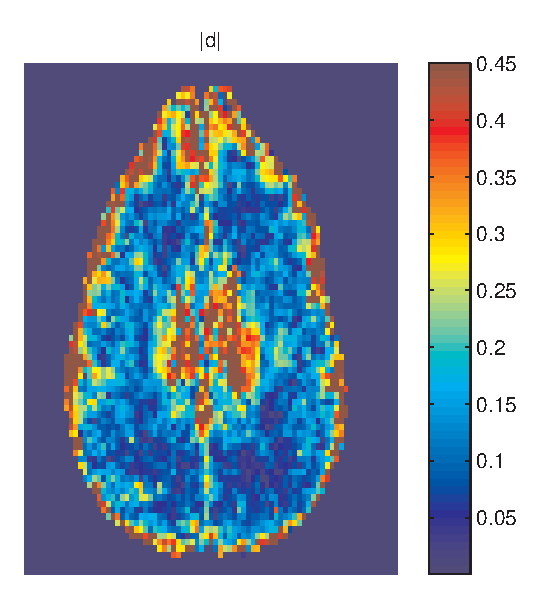
\includegraphics[width=\textwidth]{absd.eps}
      (a)
      \end{minipage}
      \begin{minipage}[]{.30\textwidth}
      \centering
      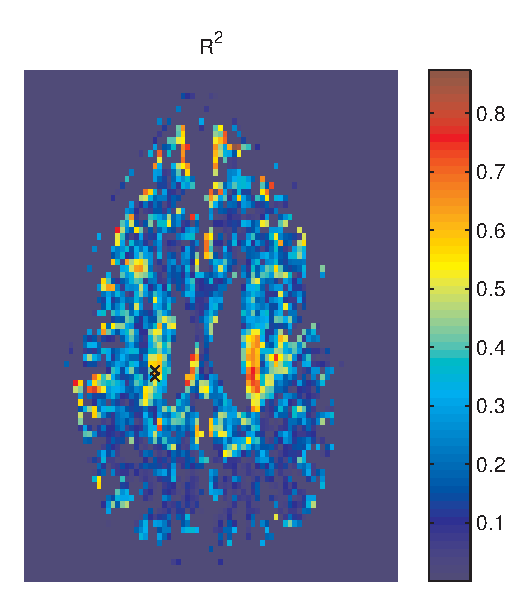
\includegraphics[width=\textwidth]{Rsqnew1typ2.eps}
       (b)
      \end{minipage}
      \begin{minipage}[]{.30\textwidth}
      \centering
      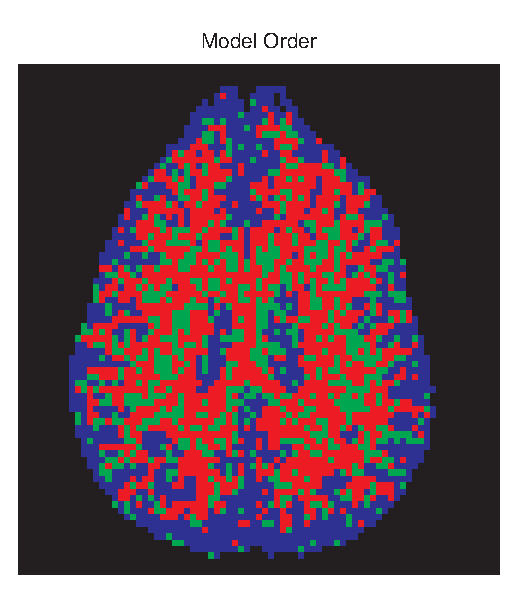
\includegraphics[width=\textwidth]{modelorderchosen2.eps}
       (c)
      \end{minipage}
      \begin{minipage}[]{.30\textwidth}
      \centering
      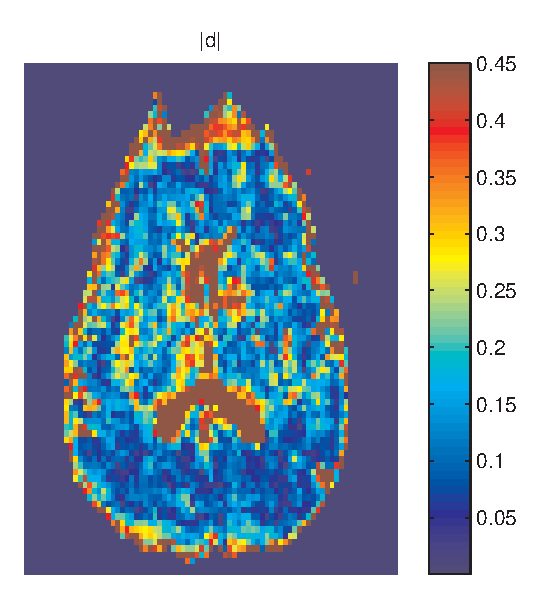
\includegraphics[width=\textwidth]{absdgg.eps}
       (d)
      \end{minipage}
      \begin{minipage}[]{.30\textwidth}
      \centering
      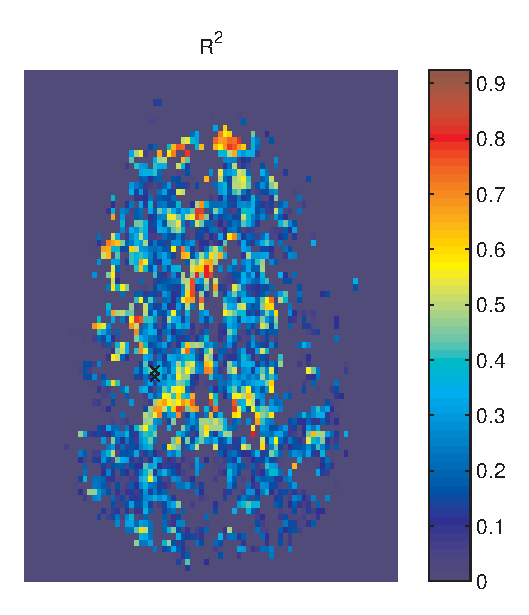
\includegraphics[width=\textwidth]{rsq255.eps}
       (e)
      \end{minipage}
      \begin{minipage}[]{.30\textwidth}
      \centering
      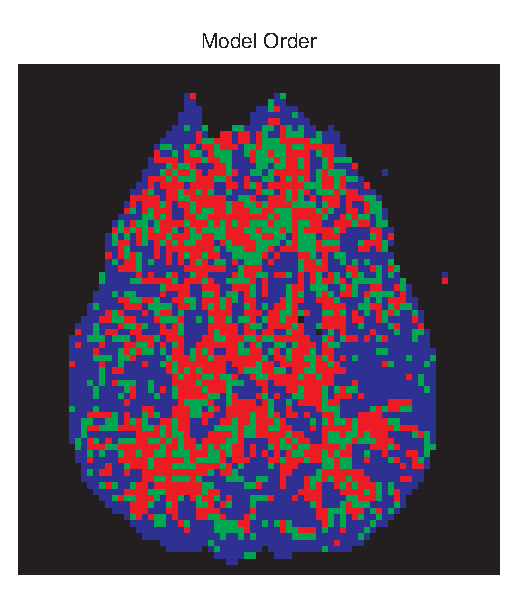
\includegraphics[width=\textwidth]{modelorderchosen2ba.eps}
       (f)
      \end{minipage}
      \begin{minipage}[]{.30\textwidth}
      \centering
      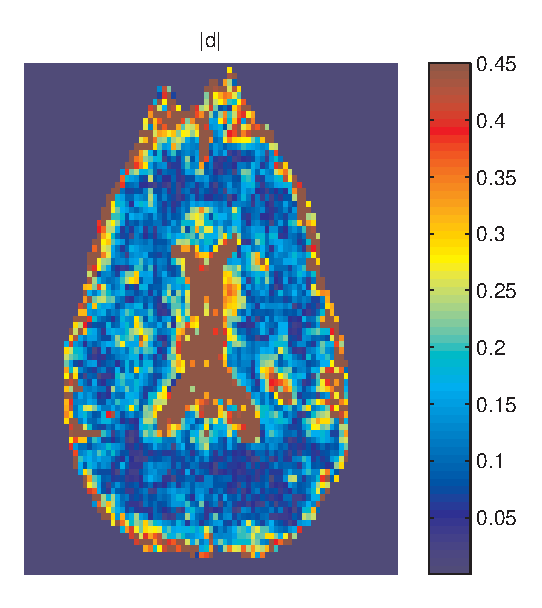
\includegraphics[width=\textwidth]{absdll2.eps}
       (g)
      \end{minipage}
      \begin{minipage}[]{.30\textwidth}
      \centering
      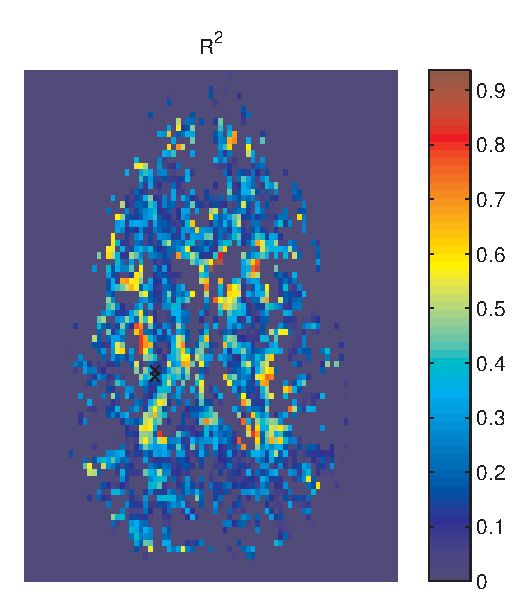
\includegraphics[width=\textwidth]{rsq255ny.eps}
       (h)
      \end{minipage}
      \begin{minipage}[]{.30\textwidth}
      \centering
      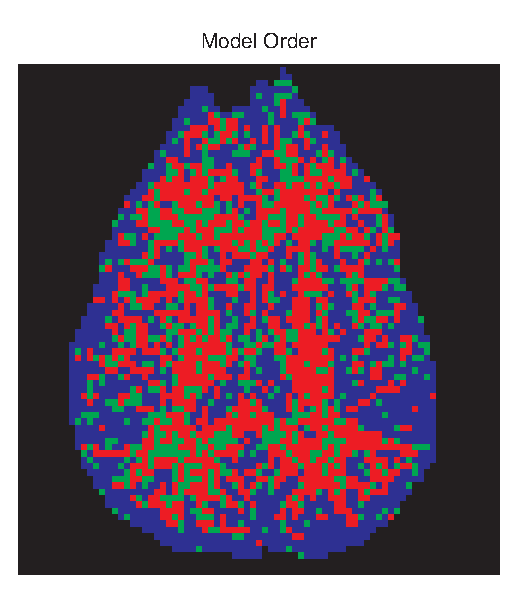
\includegraphics[width=\textwidth]{modelorderchosen2bac.eps}
      (i)
      \end{minipage}
  \end{center}
  \caption{(a, d and g) the estimated norm for the phase vector, (b, e
    and g) the goodness-of-fit value $R^2$ weighted by a one-zero
    mapping based on the FA for interpretability and (c, f, i) the
    estimated model order. The first row is slice 10, the second row
    is slice 7 and the third row is slice 8.}
  \label{fig2} 
\end{figure}
%%%%%%%%%%%%%%%%%%%%%%%%%%%%%%%%%%%%%%%%%%%%%%%%%%%%%%%%%%%%%%%%%%%%%%

%%%%%%%%%%%%%%%%%%%%%%%%%%%%%%%%%%%%%%%%%%%%%%%%%%%%%%%%%%%%%%%%%%%%%%%
\begin{figure}[tbp]
  \begin{center}
    \begin{minipage}[]{.32\textwidth}
      \centering
      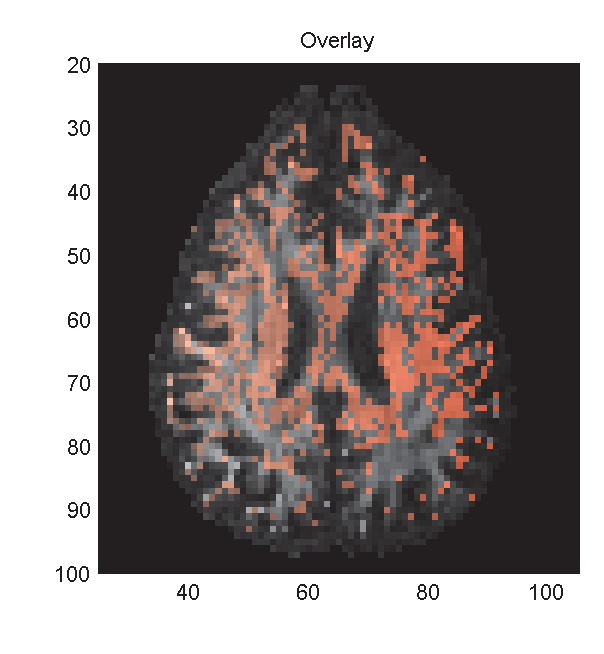
\includegraphics[width=\textwidth]{rejected.eps}
      (a)
    \end{minipage}
    \begin{minipage}[]{.32\textwidth}
      \centering
      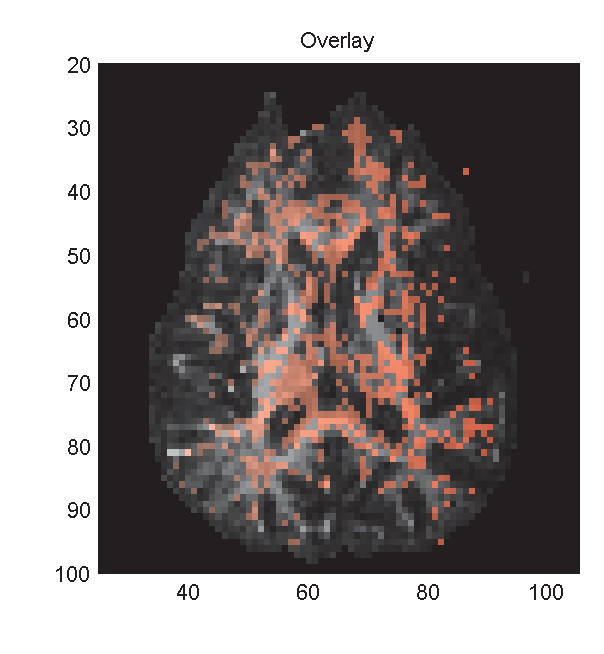
\includegraphics[width=\textwidth]{overlaynew55b.eps}
      (b)
    \end{minipage}
    \begin{minipage}[]{.32\textwidth}
      \centering
      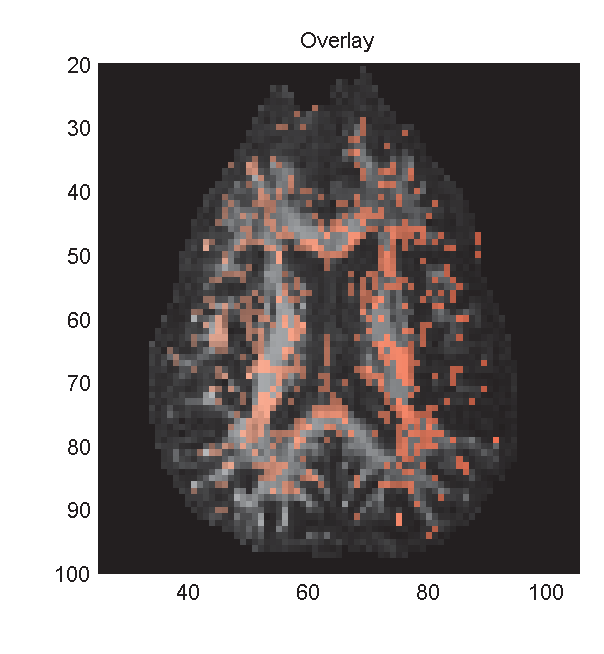
\includegraphics[width=\textwidth]{overlaynew55ny.eps}
      (c)
    \end{minipage}
  \end{center}
  \caption{Three slices from the clinical data acquisition, where
    voxels highlighted in red provide indicate strong Hermitian
    structure and the average phase is zero.}
  \label{fig3b} 
\end{figure}
%%%%%%%%%%%%%%%%%%%%%%%%%%%%%%%%%%%%%%%%%%%%%%%%%%%%%%%%%%%%%%%%%%%%%%

We show the main directions of the real magnitude (associated with the
largest eigenvalue) and the gradient of the estimated linear phase in
Figs.~\ref{fig1}(a)--(d), \ref{fig1b}(a)--(d), and
\ref{fig1c}(a)--(d), all weighted by the FA.  In all three figures we
have used either (c) a $p$-value of 0.1 to determine whether average
phase is zero, combined with the FDR procedure with $p=0.01$ on the
gradient of the phase in the retained voxels, or (d) no check on the
average phase and a non-adjusted $p$-value of 0.1 for testing the
gradient of the phase.
% We have in subplots (c) and (d) used either a 0.1 $p$-value
% procedure used with FDR, combined with FDR on the average phase at
% 0.01, or no check on the average phase and a non-adjusted $0.1$
% p-value for (d) in all the three figures.  
We show the magnitude of the phase vector (Figs.~\ref{fig2}(a,d,g))
and the $R^2$ associated with fitting the linear phase factor
(Figs.~\ref{fig2}(b,e,h)), as well as the estimated model order
(Figs.~\ref{fig2}(c,f,i)).  We apply the false discovery rate (FDR)
procedure for multiple comparisons
\citep{Benjamini,gen-laz-nic:thresholding} to determine which voxels
have an average phase equal to zero, but exhibit linear structure
(Fig.~\ref{fig3b}).
%An example of bending appears to be
%present and is marked by two crosses in Figure \ref{fig3b}(b).  We see
%that the parametric real model favours a single tensor in one case:
%fully consistent with a bending fibre on 30 measurements, and a double
%tensor in the second case.  Zooming in, we have a cluster of voxels
%where the Hermitian structure is non-negligible and the model order is
%one, \ref{fig3b}(c) and \ref{fig3b}(d).  We can also look at the $R^2$
%and the direction of the local asymmetry; i.e., \ref{fig3b}(e) and
%\ref{fig3b}(f).  The orientation seems to be green (i.e. in the $x_2$
%direction) and it is bending left/right.  We therefore plot the raw
%$q$-space structure in Fig.~\ref{fig6} for the two marked voxels,
%both with $R^2=0.64$ (note that by $R^2$ we are only looking at the
%variation explained by a linear phase, not the small constant factor
%or higher order terms.
% (see section \ref{stattest})).  
%The anticipated Hermitian structure is clearly visible from these two
%voxels, and should be compared with Fig.~\ref{bending}. 
It would appear that we have identified some bending structure,
bending left/right.  Note that the three-dimensional plots have been
rotated for better view (consistently per voxel), and so the phase
structure in Fig.~\ref{fig6} does not admit direct interpretation from
the image (see instead \ref{fig3b}(f)).  \textbf{[Contrast
    Figure~\ref{fig3b}a with Fig.~13 in \citet{jon:studying}.]}

%%%%%%%%%%%%%%%%%%%%%%%%%%%%%%%%%%%%%%%%%%%%%%%%%%%%%%%%%%%%%%%%%%%%%%
\begin{figure}[!htbp]
  \begin{center}
    \begin{tabular}{c|cccc}
      & (i) & (ii) & (iii) & (iv)\\
      \hline
      \\
      (a) & \includegraphics[width=0.2\textwidth]{73100.ps} &
      \includegraphics[width=0.2\textwidth]{73101.ps} &
      \includegraphics[width=0.2\textwidth]{73102.ps} & 
      \includegraphics[width=0.2\textwidth]{73103.ps}\\
      \\
      (b) & \includegraphics[width=0.2\textwidth]{73104.ps} &
      \includegraphics[width=0.2\textwidth]{73105.ps} &
      \includegraphics[width=0.2\textwidth]{73106.ps} & 
      \includegraphics[width=0.2\textwidth]{73107.ps}
    \end{tabular}
  \end{center}
  \caption{Two voxels of clinical data from the same axial slice in
    Fig.~\ref{fig3b}.  For both voxels the columns denote the (i)
    phase, (ii) magnitude of the real part of the complex-valued
    signal, (iii) the magnitude of the imaginary part of the
    complex-valued signal and (iv) the amplitude of the complex-valued
    signal.  For both voxels provided here the phase displays
    asymmetry similar to \textbf{???}, with an $R^2=0.64$.}
  \label{fig6}
\end{figure}
%%%%%%%%%%%%%%%%%%%%%%%%%%%%%%%%%%%%%%%%%%%%%%%%%%%%%%%%%%%%%%%%%%%%%%

\section{Discussion}
\label{discussion}

\textbf{What have we done?}  There is phase information in DW-MRI.
This information is ``free'', and neglecting the information leads to
inefficient estimation.

When the spurious phase has been removed, structure remains.  This has
to do with overall diffusion asymmetries, and allows us to recognize
bending and (hypothetically) forking structure.  In the case of
bending, it is anticipated that a linear approximation to the phase
would be sufficient, and the data does confirm this to be the case,
with an observed $R^2$ of nearly 0.8 in some cases.

\textbf{What does it do?}  This information identifies local
symmetries such as bending or forking, and we can locally describe
bending well.

\textbf{What is usually done?}  The Gaussian diffusion model has
greatly facilitated automated analysis of DTI data.  Naturally, there
are limitations in the types of white-matter microstructure that can
be described by the Gaussian diffusion model.  Crossing fibers, and
other higher-order structures, do not agree with the simple model and
produce mixed results in terms of common scalar statistical summaries;
e.g., fractional anisotropy.  Methodological developments provide a
variety of methods and models beyond the Gaussian diffusion model;
e.g., tensor mixtures, DOT, PAS-MRI, spherical deconvolution, etc.  A
line of investigation has looked at diffusion kurtosis, and higher
order properties of the PDF; e.g., diffusion kurtosis imaging
\citep{Jensen2005}.

Another possible non-Gaussian structure is asymmetry, associated with
bending and forking.  A Gaussian distribution is always symmetric,
whilst some typical features of a PDF cannot be encompassed by a
symmetric distribution.  To detect asymmetries it is necessary to
collect complex-valued observations.

\subsection{The importance of pre-processing}

The analysis of such observations is unfortunately not trivial:
initially various spurious phase effects must be removed.  Such
removal can be unsuccessful in which case subsequent analysis becomes
highly questionable.  It is therefore necessary to start after such
effects have been removed by testing if the remaining phase structure
is Hermitian symmetric.

\subsection{Strengths and weaknesses}

However, single-shell data is unlikely to yield sufficient phase
information, and as when employing higher-order tensor models, more
data are needed to fit the models. \textbf{We have done the best with
  a single shell of data!}

\subsection{Applications}

The phase information can be used to improve parametric DW-MRI
analysis methods.

With phase information, various tracking algorithms could be improved,
in a similar manner to using the scalene structure of diffusions
\citep{Seunarine}.  The advantage of the complex-valued information is
that we get an estimated orientation of the bending, and this can be
feed directly into the tracking algorithm.  For forking structure a
simple linear phase will not do, see Fig.~\ref{bending}.  In this case
we anticipate a small value of $R^2$ will indicate voxels in which the
assumption of linear phase will be insufficient.  We cannot however
fit such models from a single shell, and must collect more complicated
data to be able to deduce such structure.

\section*{Acknowledgements}

The authors would like to thank...

\appendix

\section{Data pre-processing}
\label{preprocessing:step1}

\subsection{Individual voxel/gradient/coil model}
\label{modelA1}

We write the observed signal at spatial location $\x_n$, coil $\gamma$
and diffusion sensitisation gradient $\q_j$ (unit vector) as
\begin{eqnarray}
  Z_{\gamma}(\q_l;\x_n) &=& X_{\gamma}(\q_l;\x_n) - i Y_{\gamma}(\q_l;\x_n)\\
  &=& A_{\gamma}(\q_l;\x_n) s_{\gamma}(\q_l;\x_n)
  \exp\left(-i\phi_{\gamma}(\q_l;\x_n)\right)\\
  &=&\cZ_{\gamma}(\q_l;\x_n)+\eps_{\gamma}(\q_l;\x_n)
\end{eqnarray} 
where $\gamma=1,\dots,n_{\gamma}$ and $l=1,\dots,L$.  We refer to
$A_{\gamma}(\q_l;\x_n)$ as the observed amplitude, $s_{\gamma}(\q_l;\x_n)$
is the observed coil sensitivity and $\phi_{\gamma}(\q_l;\x_n)$ is the
observed phase.
%Only the observed amplitude is really useful in its own right. 
These are also unfortunately noisy observations, contaminating the
noise-free observations
\begin{equation}
\cZ_{\gamma}(\q_l;\x_n)=\cA(\q_l;\x_n)\varsigma_{\gamma}(\q_l;\x_n)
\exp\left(-i\varphi_{\gamma}(\q_l;\x_n)\right)
\end{equation} 
by Gaussian proper noise \citep{Picinbono1996},
$\eps_{\gamma}(\q_l;\x_n)$.  We refer to $\cA(\q_l;\x_n)$ as the
(true) amplitude, $\varsigma_{\gamma}(\q_l;\x_n)$ as the (true) coil
sensitivity and $\varphi_{\gamma}(\q_l;\x_n)$ as the (true) phase.
The IFT of $\cZ_{\gamma}(\q_l;\x_n)$ is denoted $a_{\gamma}(\x;\x_n)$.
We model the variance as given by
\begin{equation}
  \var\{\eps_{\gamma}(\q_l;\x_n)\}=\sigma^2(\x_n), \quad \forall \gamma,\,l.
\end{equation}
This means that we model the variance as evolving spatially but as
staying fixed across coils $\gamma$ and orientations ${\q}_l$.  This
is equivalent to considering the main source of noise as physiological
rather than thermal (thermal noise is known to be coil dependent).  We
also assume that $\{\gamma\}$ has been chosen so that
\begin{equation}
\sum_{\gamma} \varsigma_{\gamma}(\q_l;\x_n)=C,
\end{equation}
some constant.

%We let the spatial shifts be denoted by $\bs{\tau}(\x)$ and thus
%write:
%\begin{eqnarray}
%  Z_{\gamma}(\q_l;\x) = \cA(\q_l;\x+\bs{\tau}(\x);\bld{D})
%  \varsigma_{\gamma}(\q_l;\x+\bs{\tau}(\x))
%  \exp\left(-i\varphi_{\gamma}(\q_l;\x+\bs{\tau}(\x))\right) +
%  \epsilon_{\gamma}(\q_l;\x).
%\end{eqnarray}
%  We assume that
%$\cA(\q_l;\x+\bs{\tau}(\x);\bld{D})$ is a slowly varying function, so
%that $\cA(\q_l;\x+\bs{\tau}(\x);\bld{D})\approx\cA(\q_l;\x;\bld{D})$
%and also that $\varsigma_{\gamma}(\q_l;\x+\bs{\tau}(\x))\approx
%\varsigma_{\gamma}(\q_l;\x)$.  This of course implies that
%\begin{equation}
%  Z_{\gamma}(\q_l;\x) = \cA(\q_l;\x;\bld{D})
%  \varsigma_{\gamma}(\q_l;\x) \exp\left(-i\varphi_{\gamma}(\q_l;\x +
%  \bs{\tau}(\x))\right) + \epsilon_{\gamma}(\q_l;\x).
%\end{equation}

\subsection{Modelling rigid motion}
\label{model_rigid}

With the model of Section~\ref{modelA1}, we intend to determine the
motion artifacts and remove these from the observations.  We start by
processing the observations at a fixed slice position $x_3$ and fixed
coil $\gamma$ as well as gradient direction $l$, thus only dealing
with functions in the plane of $(x_1,x_2)$.  If we shift the image by
$\x^{(o)}=(x_1^{(o)},\;x_2^{(o)})^T$ in the $(x_1,\,x_2)$ plane then
the $\q$ space representation changes by
\begin{eqnarray}
  \cZ^{\x^{(o)}}_{\gamma}(\q_l;\x_n) &=& \int\int\int
  a_{\gamma}\left(\y-\x^{(o)};\x_n\right) \exp\left(-2i\pi
  \q_l^T\y\right) \; d^3\y \nonumber\\ 
  &=& \exp\left(-2i\pi \q_l^T \x^{(o)}\right)\cZ_{\gamma}(\q_l;\x_n).
\end{eqnarray}
$\x^{(o)}$ is implicitly a function of $\x_n$.  Thus the motion will
imply a linear phase shift by $\x^{(o)}$.  However the motion is not
quite rigid, and additionally motion will happen in the full $x_1$,
$x_2$ and $x_3$ space, not just the $(x_1,\,x_2)$ plane.  We therefore
deduce that the motion will approximately have the effect of the
non-linear shift operator $\cS\{ \}$ \citep{Olhede2008}
\begin{equation}\label{eq:motion_phase}
  \cS\{\cZ_{\gamma}\}(\q_l;\x_n) = \exp\left(-2i\pi
  \ol{\varphi}_{\gamma l}(\x_n)\right)\cZ_{\gamma}(\q_l;\x_n),
\end{equation}
where $\ol{\varphi}_{\gamma l}(\x_n)$ is some smooth function in
$\x_n$.  The observed motion induced phase is in fact \textit{mainly}
smooth with some jumps due to the wrap-round of the $2\pi$ modulus
observation of the $\tan^{-1}(\cdot)$ function.  Note that we model
large scale spatial effects using $\x_n$, while the small-scale
spatial variable is $\x$ the canonical variable of $\q$.

\subsection{Estimating rigid motion phase}
\label{Est_rigid}

To estimate the motion induced phase we therefore look at
Eq.~\eqref{eq:motion_phase} which suggest that the low frequency
structure of the observed data is subject to the same phase motion as
the high-frequency structure.  It therefore is reasonable to determine
this phase from the low-frequency structure of the data, and we define
with some specified smoothness level $\alpha$ a projection of the
signal to low frequencies
\begin{eqnarray*}
  \cP_{\alpha}\left\{Z_{\gamma}\right\}(\q_l;\x_n) &=&
  \ol{A}_{\gamma}^{(\alpha)}(\q_l;\x_n)
  \ol{s}_{\gamma}^{(\alpha)}(\q_l;\x_n)
  \exp\left(-i\ol{\phi}_{\gamma}^{(\alpha)}(\q_l;\x_n)\right)\\
  &=& \ol{Z}_{\gamma}^{(\alpha)}(\q_l;\x_n).
\end{eqnarray*}
This projection is associated with a fixed bandwidth $\alpha$, that we
shall assume \textit{known}, but is de-facto user tuned in this paper.
We define an estimator of the true phase as
\begin{eqnarray}
  \hat{\varphi}_{\gamma}^{(\alpha)}(\q_l;\x_n) = \phi_{\gamma}(\q_l;\x_n) -
  \ol{\phi}_{\gamma}^{(\alpha)}(\q_l;\x_n).
\end{eqnarray}
That is, at each coil, direction and location $\x_n$ we define a high
frequency phase as being the observed phase minus the phase of the
low-frequency filtered observation $\ol{Z}_{\gamma}(\q_l;\x_n)$.  The
advantage of this model is that we avoid a {\em parametric} model for
$\ol{\phi}_{\gamma}^{(\alpha)}(\q_l;\x_n)$.

\subsection{Properties of rigid motion phase}
\label{PropRigidPhase}

We shall make the assumption that $\alpha$ has been chosen
appropriately and so with $\ol{\varphi}_{\gamma l}(\x_n)$ denoting the
smooth motion induced phase and $\varphi(\q_l;\x_n)$ the observation
excess phase
\begin{eqnarray}
\E\left\{\phi_{\gamma}(\q_l;\x_n) \right\}&=&\ol{\varphi}_{\gamma l}(\x_n)+\varphi(\q_l;\x_n)\\
\E\left\{\ol{\phi}_{\gamma}^{(\alpha)}(\q_l;\x_n) \right\}&=&\ol{\varphi}_{\gamma l}(\x_n)\\
  \E\left\{\hat{\varphi}_{\gamma}^{(\alpha)}(\q_l;\x_n)\right\} &=&
 \varphi(\q_l,\x_n),
\end{eqnarray}
if the smoothing parameter $\alpha$ has been chosen correctly, so that
the procedure neither over-, nor under-smooths.  We wish to estimate
$\varphi(\q_l;\x_n)$, and thus need to combine the $\gamma$ coil
estimates over $\gamma=1,\dots,n_{\gamma}$.  This will depend on the
properties of $\hat{\varphi}_{\gamma}^{(\alpha)}(\q_l;\x_n)$ and we
determine that
\begin{eqnarray}
  \nonumber
\hat{\varphi}_{\gamma}^{(\alpha)}(\q_l;\x_n) &=&-
  \Im\left\{\ln\left(Z_{\gamma}(\q_l;\x_n)\right)\right\} +
  \Im\left\{\ln\left(\ol{Z}_{\gamma}(\q_l;\x_n)\right)\right\}\\
  \nonumber
  &=& -\Im\left\{\ln\left({\cA}(\q_l;\x_n) \varsigma_{\gamma}(\q_l;\x_n)
  \exp\left(-i\ol{\varphi}_{\gamma l}(\x_n)-i\ol{\varphi}(\q_l;\x_n)\right) +
  \epsilon_{\gamma}(\q_l;\x_n)\right)\right\}\\
  && + \Im\left\{\ln\left(\ol{\cA}(\q_l;\x_n)
  \ol{\varsigma}_{\gamma}(\q_l;\x_n)
  \exp\left(-i\ol{\varphi}_{\gamma l}(\x_n )\right) +
  \ol{\eps}_{\gamma}(\q_l;\x_n)\right)\right\}.
\end{eqnarray}
It then follows that (assuming the SNR is sufficiently large), with
$\HOT$ denoting higher order terms,
\begin{eqnarray}
  \hat\varphi_{\gamma}^{(\alpha)}(\q_l;\x_n) &=&
  \ol{\varphi}_{\gamma l}(\x_n) + \varphi(\q_l;\x_n) -
  \ol{\varphi}_{\gamma l}(\x_n) \nonumber\\
  & & -~ 
  \Im\left\{\frac{\eps_{\gamma}(\q_l;\x_n)}%
  {\exp\left(-i(\ol{\varphi}^{(\alpha)}_{\gamma l}(\x_n) + 
  \varphi(\q_l;\x_n))\right)
  \cA(\q_l;\x_n) \varsigma_{\gamma}(\q_l;\x_n)}\right. \nonumber\\ 
    & & \left.-~ \frac{\ol{\eps}_{\gamma}(\q_l;\x_n)}{\exp\left(-i\ol{\varphi}^{(\alpha)}_{\gamma l}(\x_n)\right){\ol{\cA}}(\q_l;\x_n)\ol{\varsigma}_{\gamma}(\q_l;\x_n)} 
  \right\} + \HOT \nonumber\\
  &=& \varphi(\q_l;\x_n) + \tilde{\eps}(\q_l;\x_n) + \HOT,
\end{eqnarray}
and the higher-order terms may be ignored (with sufficiently large SNR).

\subsection{Properties of the estimated phase}
\label{PropEstPhase}

Thus it follows that with $L^2$ being the area covered by the low pass
filtered version of the signal
\begin{equation}
  \E\left\{\hat\varphi_{\gamma}^{(\alpha)}(\q_l;\x_n)\right\} =
  \varphi(\q_l;\x_n) + \HOT,
\end{equation}
and so
\begin{eqnarray}
  \nonumber 
  \var\left\{\hat\varphi_{\gamma}^{(\alpha)}(\q_l;\x_n)\right\} &=&
  \frac{\sigma^2(\x_n)}{{\cA}^2(\q_l;\x_n)\varsigma_{\gamma}^2(\q_l;\x_n)} +
  \frac{\sigma^2(\x_n)}{L^2{\cA}^2(\q_l;\x_n)\varsigma_{\gamma}^2(\q_l;\x_n)}\\ 
  \nonumber
  & & - 2 \,
  \Re\left\{\frac{\sigma^2(\x_n)}{L\exp\left(i\varphi(\q_l;\x_n)\right) 
    {\cA}^2(\q_l;\x_n) \varsigma_{\gamma}^2(\q_l;\x_n)}\right\}\\ 
  \nonumber
  &=& \frac{\sigma^2(\x_n)}{{\cA}^2(\q_l;\x_n)\varsigma_{\gamma}^2(\q_l;\x_n)}
  \left(1+\frac{1}{L^2} -2 \, 
  \frac{\cos\left(\varphi(\q_l;\x_n)\right)}{L}\right).
\end{eqnarray}
We can deduce directly from the equation above that 
\begin{eqnarray*}
  \frac{\sigma^2(\x_n)}{{\cA}^2(\q_l;\x_n)\varsigma_{\gamma}^2(\q_l;\x_n)}
  \left[1-\frac{1}{L} \right]^2 &\le&
  \var\left\{\hat\varphi_{\gamma}^{(\alpha)}(\q_l;\x_n)\right\}\\
  &\le& 
  \frac{\sigma^2(\x_n)}{{\cA}^2(\q_l;\x_n)\varsigma_{\gamma}^2(\q_l;\x_n)} 
  \left[1 + \frac{1}{L}\right]^2.
\end{eqnarray*}
While we could keep the exact form -- such as given above -- for
simplicity we shall approximate the variance to be:
\begin{equation}
  \var\left\{\hat{\varphi}_{\gamma}^{(\alpha)}(\q_l;\x_n)\right\} \sim
  \frac{\sigma^2(\x_n)}{\cA^2(\q_l;\x_n) \varsigma_{\gamma}^2(\q_l;\x_n)}.
\end{equation}

\subsection{Estimating excess phase and its properties}
\label{EstExcessPhase}

To avoid a deluge of symbols in the subsequent calculations we take
\begin{equation}
  \cA_{\gamma}(\q_l;\x_n) = \cA(\q_l;\x_n) \varsigma_{\gamma}(\q_l;\x_n),
\end{equation}
this giving us one amplitude at each coil and orientation.  
We also have assumed that
\begin{equation}
  \cov\left\{\hat{\varphi}_{\gamma}^{(\alpha)}(\q_l;\x_n),
  \hat{\varphi}_{\gamma'}^{(\alpha)}(\q_l;\x_n)\right\} = 0, \quad
  \text{if} \quad \gamma \neq \gamma',
\end{equation}
or that information from different coils is independent.  We then
define aggregate (over $\gamma$) estimators at each gradient
orientation by
\begin{eqnarray}\label{aggregate}
  \wh{\cA}_{\gamma}^{(n)}(\q_l;\x_n) &=&
  \left|Z_{\gamma}(\q_l;\x_n)\right|,\\
  A(\q_l;\x_n) &=& \sum_{\gamma}\wh{\cA}_{\gamma}^{(n)}(\q_l;\x_n)\\
  \phi(\q_l;\x_n) &=& \frac{\sum_{\gamma} \wh{\cA}_{\gamma}^{(n)}(\q_l;\x_n)\hat{\varphi}_{\gamma}^{(\alpha)}(\q_l;\x_n)}{\sum_{\gamma} \wh{\cA}_{\gamma}^{(n)}(\q_l;\x_n)}\\ 
  \nonumber
  \E\left\{\phi(\q_l;\x_n)\right\} &=& \varphi(\q_l;\x_n) + \HOT\\
  \nonumber
  \var\left\{\phi(\q_l;\x_n) \right\} &= &
  \frac{\sigma^2(\x_n)}{\left[\sum_{\gamma}{\cA}_{\gamma}^{(n)}(\q_l;\x_n)\right]^2} + \HOT.  
\end{eqnarray}
The higher-order terms become important when the SNR is low.  As long
as the signal to noise ratio is sufficiently high, we find that
$\phi(\q_l;\x_n)$ is approximately Gaussian.  We can then
define
\begin{equation}
  Z(\q_l;\x_n) = A(\q_l;\x_n)\exp\left(-i\phi(\q_l;\x_n)\right),
\end{equation}
and this estimate will subsequently be treated like an observed
$Z(\q_l;\x_n)$ (Eq.~\eqref{qxeqn}) and the latter argument suppressed
for brevity and additional clarity.

\bibliographystyle{elsarticle-harv}
\bibliography{phasebib}

\end{document}
%%
%% End of file `elsarticle-template-num.tex'.
